\documentclass[11pt]{beamer}
\usepackage{beamertheme/beamerthemeJuelich}

\usepackage{appendixnumberbeamer}
\usepackage{epstopdf}
\setbeamertemplate{footer element1}[logo]{logos/BUW_Logo-schwarz}
\setbeamertemplate{frame number}[full]

\usepackage{subcaption} % subfigure
\usepackage{tcolorbox}

\usepackage{booktabs} % midrule
\usepackage{colortbl} % rowcolor
\usepackage{multirow}

\usepackage{xcolor}
\usepackage{pgfplots}
\usepackage{femtikz}
\usetikzlibrary{shapes,arrows,positioning}
\usepgfplotslibrary{colorbrewer}
\usepgfplotslibrary{groupplots}

\pgfplotsset{select coords between index/.style 2 args={
    x filter/.code={
      \ifnum\coordindex<#1\def\pgfmathresult{}\fi
      \ifnum\coordindex>#2\def\pgfmathresult{}\fi
    }
}}

\usepackage{isomath}
\newcommand{\h}{\textit{h}}
\newcommand{\p}{\textit{p}}
\newcommand{\hp}{\textit{hp}}

\newcommand{\dealii}{\texttt{deal.II}}
\newcommand{\pforest}{\texttt{p4est}}
\newcommand{\petsc}{\texttt{PETSc}}
\newcommand{\trilinos}{\texttt{Trilinos}}
\newcommand{\epetra}{\texttt{Epetra}}
\newcommand{\aztecoo}{\texttt{AztecOO}}
\newcommand{\ml}{\texttt{ML}}
\newcommand{\xsdk}{\texttt{xSDK}}

\newcommand{\opencascade}{\texttt{OpenCASCADE}}
\newcommand{\opensalome}{\texttt{OpenSALOME}}
\newcommand{\fftw}{\texttt{FFTW}}
\newcommand{\mofem}{\texttt{MoFEM}}
\newcommand{\phg}{\texttt{PHG}}
\newcommand{\phaml}{\texttt{PHAML}}


\usepackage[backend=biber, style=authoryear]{biblatex}
\addbibresource{misc/bibliography.bib}



\author{Marc Fehling~~\vrule width0.3pt~~m.fehling@fz-juelich.de}
\title{Algorithms for massively parallel generic hp-adaptive FEM}
\subtitle{\vspace{-1em}}
\titlegraphic{
  \includegraphics[height=0.37\paperheight]{figures/corner_447px.png}
  \hspace{.1em}
  \includegraphics[height=0.37\paperheight]{figures/corner-fedegrees-legendre-05_447px.png}
  \hspace{.1em}
  \includegraphics[height=0.37\paperheight]{figures/corner-subdomains-legendre-05_447px.png}
}
\date{June 05, 2020}
%\institute{Institute for Advanced Simulation (IAS)}



\begin{document}

\maketitle

\begin{frame}
\frametitle{Table of contents}
\tableofcontents
\end{frame}

\chapter{Introduction}
\label{ch:introduction}
\glsresetall

%\todo{Introduction:}
%\begin{itemize}
%  \item Need for new computational methods (adaptive)
%  \item Statistics on usage of FDS? (literatur aus bennis diss?)
%  
%  \item Latest catastrophes: tower, Düsseldorf
%  \item ... help to .. catastrophes by giving hints on placements of safety measures.
%\end{itemize}

% introduction

For the analysis of most problems in science and engineering, mathematical modeling is required to capture underlying correlations and apply findings to related variations. With rising complexity of the model, an analytical solution of a problem so described is less likely to exist, and can only be acquired via approximation with numerical methods. Computers are used today to solve these kinds of problems numerically, but depending on the complexity of the problem and the computer hardware used, such analyses can have exceptionally long execution times.

An intelligent distribution of the computing resources, which due to the dynamics of a simulation does not have to be done \textit{a priori} but progressively, can be used to reduce the computing time (\textit{strong scaling}), and to provide more accurate results in the same execution time (\textit{weak scaling}). This is possible both physically by workload distribution to several processors
% exploiting the hardware structure
and logically by
an adaptive resolution of the simulation%
% allocating resources to critical operations
, in each case based on the current state of the simulation.
Recent advancements in computer technology allows us to solve problems with billions of unknowns. However, raw computing power does not mean we can use it without further ado. Only the combination with algorithms that use all available resources efficiently and scale with the problem size offers a massive potential to reduce execution times.
%The keys to efficiency are algorithms that exploit the hardware structure and focus resources on critical operations.
The goal of this dissertation is the provision of such new, efficient algorithms.

% algorithms on hardware level

Applications can be optimized for the hardware structure up to the instruction level, for example using \gls{simd} instructions combined with vectorization, and by avoiding bottlenecks caused by memory and network bandwidth.
Furthermore, modern multi-core and multi-processor systems require parallelization to make hardware threads and processes cooperate with each other, respectively. %, which highly depends on hardware architecture.
%on which we will focus in this dissertation.
%The choice of parallelization highly depends on hardware architecture, and are a requirement for large-scale supercomputers with distributed memory access.
Depending on the hardware architecture, many different \glspl{api} have been developed over the last decades which allow developers to take opportunity of unified interfaces.
For machines with shared memory access like modern desktop workstations, independent computing tasks can be distributed among all hardware threads subjecting to a work stealing policy, for which \gls{openmp}\textsuperscript{\textregistered} \textcite{openmp50} and Intel\textsuperscript{\textregistered} \gls{tbb} \textcite{tbb2018} are the most prominent approaches.
On large-scale supercomputers, processes are spread out on multiple computing nodes with independent memory segments connected via network. To enable them to cooperate, data needs to be exchanged between all participating nodes. For communication between processes, the \gls{mpi} \textcite{mpi31} has become a standard. A hybrid combination of both techniques for shared and distributed memory is possible.
%If architecture is distributed on nodes and thus have distributed memory access, the \gls{mpi} \textcite{mpi31} will be used.
Recently, streaming multiprocessor architectures on \glspl{gpu} have become of more and more interest for scientific applications, which offer lots of theoretical throughput, but are strongly limited in flexibility. \gls{openacc}\textsuperscript{\textregistered} \textcite{openacc27} and Nvidia\textsuperscript{\textregistered} \gls{cuda}\textsuperscript{\textregistered} \textcite{cuda10} provide interfaces for the scientific use of \glspl{gpu}.

% methods for spatial discretization

Numerical methods require the discretization of the continuous space which will be divided into smaller entities that couple with neighboring ones. A large variety of these methods exist, of which we briefly describe the most commonly used ones.
With \glspl{fdm}, differential operators are evaluated as difference quotients on a finite number of grid points. %Those are easy to implement, but inflexible
The idea of \glspl{fvm} is the preservation of conserved quantities on small volumes by applying the Gauss-Ostrogradski theorem, which results in balancing volumetric averages with fluxes on interfaces of neighboring volumes.
%With the \gls{fvm}, conserved quantities are preserved on small volumes applying the Gauss-Ostrogradsky theorem, resulting in balancing volumetric averages and fluxes on interfaces.
In \glspl{fem}, we specify a function space of piecewise polynomials in which we find the function 
%is supposed to be part of, and find the representation
that minimizes the residual of the investigated problem.
%\gls{fem} contains \gls{fvm} intrinsically if you consider piecewise constant functions.

% algorithms for adaptation

In addition to optimizing numerical methods to the hardware, we can also adjust the numerical discretization to the local complexity of the investigated problem by adapting its resolution.
%we can also on a logical level by focusing computational resources on critical sections of the investigated problem.
%On the other hand, focus computational ressources on critical sections of the domain, which are problem dependet and  These sections . adaptive
This does not only assure the full utilization of all available resources, but also their efficient usage.
%The key to use those ausnutzen fully are efficient algorithms that either fit to the hardware or distribute resources on computing intensive operations.
%A combinatation of both hardware and .. software driven algorithms can be supplied. However, their combination is not trivial.
%Adaptive methods assign resolution of the problem on interesting parts of the domain.
%A common approach is adapting the numerical discretization to the specifics of the investigated problem.
With \gls{amr}, or \h-adaptive refinement, the spatial resolution of our discretization will be locally assigned, resulting in entities with different sizes $h$. While \gls{fdm} requires a regular topology for \gls{amr}, it is applicable on \gls{fvm} and \gls{fem} without major restrictions. In addition, \gls{fem} offers the unique capability for \p-adaptation, in which the polynomial degree of the basis functions is locally set. The combination of both is possible, resulting in \hp-adaptive methods.
%, which are the focus of this dissertation.

% universal application of these methods

The presented algorithms can be applied on various problems involving partial differential equations from mathematics, nature, and engineering. They have already been extensively used for e.g.\@ structural mechanics, heat transfer, wave propagation, electrostatics, and fluid dynamics to name just a few.
In engineering practice, these methods form the basis for simulations on objects, for instance to investigate their stress and wear behavior and to generate their flow profile. Corresponding model experiments are complex and expensive, so computer simulations offer an alternative.
A concrete application example describes the simulation of smoke spread in buildings.
On basis of their results, fire safety engineers are able to optimize smoke extraction systems and evacuation routes to increase the safety of civilians in the event of a fire outbreak.
In general, fires remain spatially localized even after their ignition phase, so the dynamic allocation of both resolution and computational resources is highly favorable in this scenario.
Their simulation on large scale buildings or connected facilities like underground tunnel systems as investigated in the ORPHEUS project \parencite{arnold2017}, yield an incredible amount of workload.
%a use of adaptive methods . and the combination with parallelization on large-scale buildings, or even large connected facilities like underground stations as investigated in the \texttt{ORPHEUS} project, yield a lot of complexity and thus a lot of workload.

%Further, the combination of an efficient use of computational ressource via parallelization as well as an intelligent assignment of these ressource on crucial areas of the problem via adaptation is incredibly important.

Thus, the combination of parallelization and adaptive methods is necessary to perform simulations on an economically acceptable time scale. However, their implementation is very difficult with lots of technical finesses to consider.
%The combination of both parallelization with adaptative methods is necessary is highly favorable, but very difficult to implement with lots of technical finesses to consider.
%Both methods require lots of technical finesses to make them availble. as well as mathematical ... .
%Although there are many software solutions that offer parallel \h-adaptive methods, only a few offer \hp-adaptive methods and even less combine it with parallelization.
Many software solutions for parallel \h-adaptive methods exist, however their \hp-adaptive equivalents are rarely realized because of their complexity.
In this dissertation, we will focus on \hp-adaptive \gls{fem} with their exceptional error convergence properties \parencite{guo1986,babuska1996}, and provide their parallelization for distributed memory systems.
%This thesis presents the combination of both parallelization on distributed hardware architecture, and hp-adaptive methods.

% existing software solutions

%\textcite{shahbazi2007}

In the past, several algorithms for parallel \hp-adaptive \gls{fem} have been developed, but they always stayed in the context of \gls{dg} methods which allow solutions to be discontinuous across cell interfaces. For example for Navier-Stokes problems, \textcites{paszynski2006}{chalmers2019} presented methods for distributed memory architectures, while \textcites{paszynski2011}{jomo2017} demonstrated methods for shared memory machines. A general approach which also works with \gls{cg} methods poses additional implementation challenges that are pointed out in the course of this dissertation. %and has not been published yet.

%\textcite{paszynski2006}
% demkovisz par

Due to their complexity, \hp-adaptive methods have always stayed in an experimental stage and have never been prepared to be easily applied by a broader academic audience, especially in combination with parallelization.
Though, there are several open-source libraries available to the public that provide the bare functionality for \hp-adaptive \gls{fem} on distributed memory architectures using the \gls{mpi} protocol, such as the libraries \phaml{} \parencite{mitchell2002,phaml1200}, \phg{} \parencite{zhanglin-bo2019,phg094}, and \mofem{} \parencite{kaczmarczyk2020,mofem090}. However, even here the application of these features is not immediately accessible to the end user. We are not aware of any commercial tools capable of this feature.

% par3dhp - not publicly available
% hermes - only openmp parallelization

% deal.II

%Further, although parallel \hp-adaptive \glspl{fem} have been presented thoroughly, there is no systematic description on how to realize them yet as a software application. There are publications that highlight all necessary data structures and algorithms parallelization \parencite{bangerth2012} (parallel paper) and \hp-adaptive methods \parencite{bangerth2009}.

Furthermore, although applications of parallel \hp-adaptive \glspl{fem} have been presented thoroughly, there is no systematic description on how to realize them yet as a software implementation.
Algorithms and data structures have already been presented in detail for parallel \h-adaptive \gls{fem} by \textcite{bangerth2012} and sequential \hp-adaptive \gls{fem} by \textcite{bangerth2009}.
%However, the combination of both elaborations is not trivial and has not yet been carried out.
The goal of this dissertation is to provide the combination of both algorithms highlighting difficulties to combine both parallelization with \hp-adaptive methods. This dissertation is not meant to be an in-depth guide for the creation of \gls{fem} software. We would rather like to emphasize on the basic ideas for parallel \hp-adaptive \gls{fem} and point out programming challenges. We will provide an example implementation in the \dealii{} library \parencite{bangerth2007, dealii920pre}, so that the reader is able to either embed our findings into their own \gls{fem} code or use the \dealii{} implementation right away.

\dealii{} is an open-source software library for the creation of general purpose \gls{fem} codes.
%It offers lots of additional features for \gls{fem} that go beyond usual
%With it, users can easily generate their own application for scientific research on basis of the expertise of their developers.
It is part of the \gls{xsdk} \parencite{bartlett2017,xsdk050},
%and builds upon interfaces to other libraries providing .
which combines efforts of many research software engineers to make their expertise in optimized \gls{hpc} available and provides them to the public as a whole.
%and combine it with to all packages in this kit
%from which all packages in this kit profit.
%share their own expertise and benefit from others
%It is a joint effort to provide a set of tools for exascale computing.
%relying on the expertise of other developers and their
%and offers lots of features
In this context of sharing knowledge, \dealii{} profits from parallel linear algebra provided by the open-source libraries \trilinos{} \parencite{heroux2005,trilinos12181} and \petsc{} \parencite{balay2019,petsc3124}, and utilizes their implementation via designated interfaces.
%In the \dealii{} library, we rely on third party libraries. Parallel linear algebra by \trilinos{} \parencite{heroux2005,trilinos12181} and \petsc{} \parencite{balay2019,petsc3124}.

Furthermore, \dealii{} does not provide the hierarchic generation of \h-adaptive meshes and their partitioning on multiple processes of distributed memory architectures itself, but relies on the implementation of the open-source library \pforest{} \parencite{burstedde2011,p4est22}. In this regard, \pforest{} is used as an `oracle': Operations that manipulate the mesh and its partitioning happen on a distributed structure provided by \pforest{}, and will be recreated only on the locally owned sections of the \dealii{} mesh
%and data structures
on every process with a set of queries to the master mesh.
%Every cell related data is thus stored in both libs in the very same way. They both use Z-order or Molten-schemes to iterate over cells. (sth like that?)

Since the ideas of this dissertation will be realized in \dealii{}, we capitalize on their hierarchic quadtree and octree structures with corresponding quadrilateral and hexahedral cells in two and three dimensions, which are arranged by means of a Z-order or Morton space-filling curve.
%The combination of \dealii{} and \pforest{} poses restrictions based on decisions made during their development process, for example the specialization on hierarchic quadtree and octree structures with corresponding quadrilateral and hexahedral cells in two and three dimensions, which will be arranged by means of a Z-order or Morton space-filling curve.
%Although the combination of \dealii{} and \pforest{} relies on quadrilateral and hexahedral cells in two and three dimensions for which they use a Z-order or Morton scheme
However, the presented ideas for algorithms and data structures in this dissertation are not restricted to these specifications.

% thesis outline

%Algorithms and data structures have already been presented for parallel \h-adaptive \gls{fem} by \textcite{bangerth2012} and sequential \hp-adaptive \gls{fem} by \textcite{bangerth2009}. However, the combination of both elaborations is not trivial.

In this dissertation, we present all enhancements necessary to supply parallel \hp-adaptive methods for algorithms and data structures that are already capable of parallel \h-adaptive and sequential \hp-adaptive \gls{fem}. In Ch.~\ref{ch:parallel} we present the necessary details for static meshes, i.e.\@ meshes with fixed resolution and assignment of finite elements from beginning to end of a simulation. Ch.~\ref{ch:dynamic} deals with all necessities of dynamic \hp-adaptive methods, and presents algorithms to automatically determine regions to adapt. We apply the presented methods on a simple numerical example in Ch.~\ref{ch:results} to show the benefits of \hp-adaptive methods and the scalability on the JURECA supercomputer \parencite{krause2016,jureca}.

Some of the algorithms presented in this dissertation have already been published in the current release of the \dealii{} library \parencite{arndt2019} and their entirety will be made available completely with the upcoming release. All numerical examples in this dissertation have been performed using a certain version of the library published on a public fork \textcite{finaldissertation} of the corresponding \dealii{} repository \textcite{dealii920pre}.

\section{hp-adaptive methods}





\begin{frame}
\frametitle{Table of contents}

\tableofcontents[currentsection]
\end{frame}





\subsection{Finite Element Method}





\begin{frame}
\frametitle{Finite element method}

\begin{minipage}{.59\textwidth}
  \begin{itemize}
  \item Shape functions form nodal basis
    \begin{align*}
    \varphi_i(x_j) = \delta_{ij} =
    \begin{cases}
    1 & \text{for} ~ i=j \\
    0 & \text{for} ~ i \neq j
    \end{cases}
    \end{align*}
  \item $Q_p$ elements from Lagrange interpolation with degree $p$
  \end{itemize}
  
  \vspace{1em}
  
  \begin{itemize}
  \item Finite element approximation is linear combination of shape functions
    \begin{align*}
    u_{hp}(x) = \sum_i \, u_i \, \varphi_i(x)
    \end{align*}
  \item Coefficients $u_i$ are degrees of freedom
  \end{itemize}
\end{minipage}
\hfill
\begin{minipage}{.4\textwidth}
  \vspace{-1em}
  
  \begin{figure}
  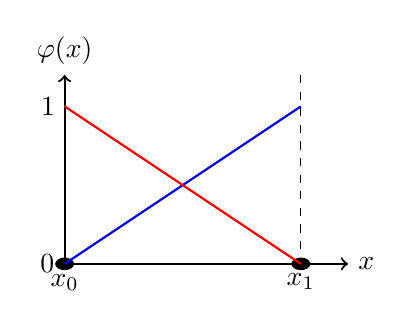
\begin{tikzpicture}[scale=2, xscale=1.5]
  % Draw axes
  \draw [<->,thick] (0,0) node [below] {$x_0$} node[left] {0}
  (0,1.2) node (yaxis) [above] {$\varphi(x)$}
  |- (1.2,0) node (xaxis) [right] {$x$};
  
  % Draw dashed
  \draw [dashed] (1,1.2) -- (1,0) node [below] {$x_1$};
  
  % Draw nodes
  \foreach \x in {0,1} {
    \fill (\x,0) circle (.04cm);
    %\fill (\x,1) circle (.04cm);
  }
  \node[left] at (0,1) {1};
  
  % Draw functions
  \draw[thick,color=blue,domain=0:1] plot (\x,{\x});
  \draw[thick,color=red,domain=0:1] plot (\x,{1-\x});
  \end{tikzpicture}
  \vspace{-0.8em}
  \caption{$Q_1$ element}
  \end{figure}
  
  \vspace{-2.5em}
  
  \begin{figure}
  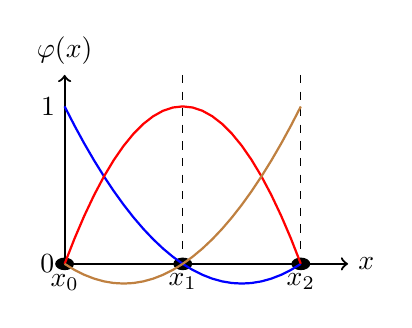
\begin{tikzpicture}[scale=2, xscale=1.5]
  % Draw axes
  \draw [<->,thick] (0,0) node [below] {$x_0$} node[left] {0}
  (0,1.2) node (yaxis) [above] {$\varphi(x)$}
  |- (1.2,0) node (xaxis) [right] {$x$};
  
  % Draw dashed
  \draw [dashed] (0.5,1.2) -- (0.5,0) node [below] {$x_1$};
  \draw [dashed] (1,1.2) -- (1,0) node [below] {$x_2$};
  
  % Draw nodes
  \foreach \x in {0,0.5,1} {
    \fill (\x,0) circle (.04cm);
    %\fill (\x,1) circle (.04cm);
  }
  \node[left] at (0,1) {1};
  
  % Draw functions
  \draw[thick,color=blue,domain=0:1] plot (\x,{2*\x*\x - 3*\x + 1});
  \draw[thick,color=red,domain=0:1] plot (\x,{(-4)*\x*\x + 4*\x});
  \draw[thick,color=brown,domain=0:1] plot (\x,{2*\x*\x - \x});
  \end{tikzpicture}
  \vspace{-0.8em}
  \caption{$Q_2$ element}
  \end{figure}
\end{minipage}
\end{frame}





\subsection{Adaptive methods}





\begin{frame}
\frametitle{Adaptive methods}

\begin{itemize}
\item Focus computational resources on areas of interest
\item Align simulation resolution with complexity of current solution
\end{itemize}

\vfill{}

\begin{itemize}
\item Finite Element Method (FEM) provides two different possibilities:
\begin{tabular}{lll}
  \textbf{\h}-adaptation: & dynamic cell sizes & good for irregular solutions \\
  \textbf{\p}-adaptation: & dynamic function spaces & good for smooth solutions
\end{tabular}
\item Combination of both possible
\end{itemize}

\vfill{}

\begin{minipage}{.49\textwidth}
  \begin{figure}
  \begin{tikzpicture}[scale=2.2]
  \def\Length{0.5}
  \def\Radius{0.03}
  
  \LagrangeCell{-2*\Length}{0}{2*\Length}{\Radius}{2}
  {{,,,,,,,,}};
  
  % remove face node which becomes a hanging node on a vertex
  \draw[fill=white,draw=white] (0,\Length-\Radius) rectangle (-\Radius,\Length+\Radius);
  
  \LagrangeCell{0}{0}{\Length}{\Radius}{2}
  {{,,,,,,,,}};
  \LagrangeCell{\Length}{0}{\Length}{\Radius}{2}
  {{,,,,,,,,}};
  \LagrangeCell{0}{\Length}{\Length}{\Radius}{2}
  {{,,,,,,,,}};
  \LagrangeCell{\Length}{\Length}{\Length}{\Radius}{2}
  {{,,,,,,,,}};
  \end{tikzpicture}
  \caption{\h-adaptivity}
  \end{figure}
\end{minipage}
\begin{minipage}{.49\textwidth}
  \begin{figure}
  \begin{tikzpicture}[scale=2.2]
  \def\Length{1}
  \def\Radius{0.03}
  
  \LagrangeCell{0}{0}{\Length}{\Radius}{2}
  {{,,,,,,,,}};
  \LagrangeCell{\Length}{0}{\Length}{\Radius}{4}
  {{,,,,,,,,,,,,,,,,,,,,,,,,}};
  \end{tikzpicture}
  \caption{\p-adaptivity}
  \end{figure}
\end{minipage}
\end{frame}





\begin{frame}
\frametitle{Adaptation criteria}

\begin{itemize}
\item \textbf{Which} cells to adapt?
\item \textbf{How} to adapt? \h/\p?
\end{itemize}

\pause
\vfill{}

\begin{itemize}
\item Manual adaptation
\item Automatic adaptation
  \begin{itemize}
  \item Criterion to indicate adaptation
  \item General approach -OR- tied to the problem
  \end{itemize}
\end{itemize}

\pause
\vfill{}

\begin{itemize}
\item Automatic \hp-decision strategies discussed in the dissertation
  \begin{enumerate}
  \item Error prediction based on refinement history \newline \parencite{melenk2001}
  \item Smoothness estimation by decay of Fourier coefficients \newline \parencite{bangerth2009}
  \item Smoothness estimation by decay of Legendre coefficients \newline \parencite{mavriplis1994}
  \end{enumerate}
\end{itemize}
\end{frame}





\subsection{Example: Laplace equation}





\begin{frame}
\frametitle{Example: Reentrant corner}

\begin{minipage}{.47\textwidth}
\begin{itemize}
  \item Singularity at reentrant corners for elliptic problems
  \item L-shaped domain:
    \begin{align*}
    \Omega = [-1,1]^2 \setminus \left([0,1]\!\times\![-1,0]\right)
    \end{align*}
  \item Manufactured Laplace problem
    \begin{align*}
    - \nabla^2 u &= 0 \qquad\text{on}\quad \Omega \\
    u &= \bar{u} \qquad\text{on}\quad \partial\Omega \\[.5em]
    \bar{u} &= r^{2/3} \, \sin\left(2/3 ~ \varphi\right) \\
    \|\nabla \bar{u}\| &= r^{-1/3}
    \end{align*}
\end{itemize}
\end{minipage}
\hfill{}
\begin{minipage}{.51\textwidth}
  \begin{figure}
  \resizebox{\textwidth}{!}{
    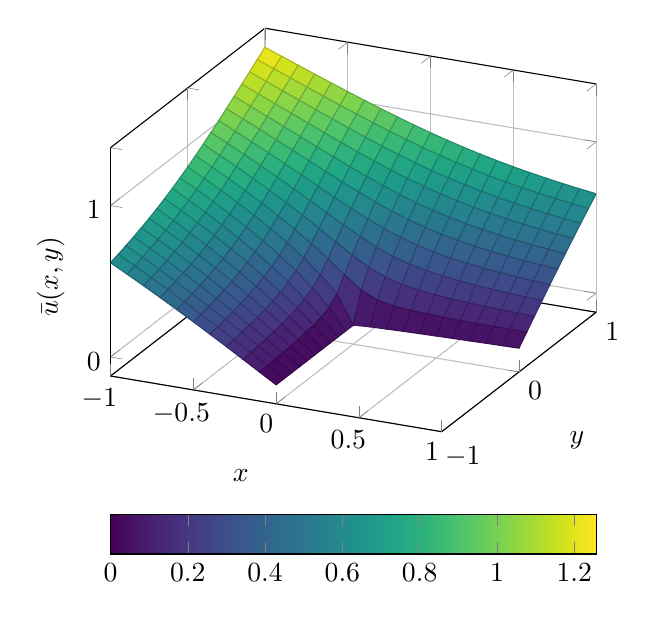
\begin{tikzpicture}
    \begin{axis}[
    scale=0.9,
    grid=major,
    colorbar horizontal,
    colormap/viridis,
    xlabel=$x$,
    ylabel=$y$,
    zlabel={$\bar{u}(x,y)$}
    ]
    \addplot3[
    surf,
    domain=-1:1,
    y domain=-1:1,
    restrict expr to domain={(x>0)&&(y<0)}{0:0},
    samples=21
    ]{pow(x*x+y*y,0.33)*sin(0.66*(atan2(y,-x)+90)))};
    \end{axis}
    \end{tikzpicture}
  }
  \caption{L-shaped domain}
  \end{figure}
\end{minipage}
\end{frame}





\begin{frame}
\frametitle{Example: Successive refinement}

\begin{itemize}
\item Initialize coarse mesh
\item Solve and refine in multiple cycles for tailored discretization
\end{itemize}

\begin{figure}
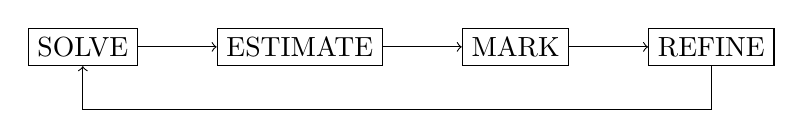
\begin{tikzpicture}[block/.style={draw}]%, node distance=.35cm]
\node [block] (solve) {SOLVE};
\node [block, right=of solve] (estimate) {ESTIMATE};
\node [block, right=of estimate] (mark) {MARK};
\node [block, right=of mark] (refine) {REFINE};

\draw[->] (solve) -- (estimate);
\draw[->] (estimate) -- (mark);
\draw[->] (mark) -- (refine);
\draw[->] (refine) -- ($ (refine) + (0,-0.8) $)  -| (solve);
\end{tikzpicture}
\caption{Successive refinement}
\end{figure}

\begin{enumerate}
\item Calculate refinement criteria (here: error estimates)
\item Flag 30\%/3\% of cells with highest/lowest criterion for refinement/coarsening
\item Calculate decision criteria (here: smoothness estimates)
\item Flag 90\%/10\% for $p$-/$h$-adaptation
\end{enumerate}
\end{frame}





\begin{frame}
\frametitle{Example: Successive refinement}

\begin{figure}
\only<1>{
  \begin{tikzpicture}
  \begin{axis}[
  scale=1,
  xmin=-1,xmax=1,
  ymin=-1,ymax=1,
  unit vector ratio={1 1},
  tick align=outside,
  xlabel=$x$,
  ylabel=$y$,
  colormap/OrRd,
  colorbar sampled,
  colorbar style={ylabel={finite element polynomial degree}, samples=7, ytick={2,3,...,7}},
  colormap access=piecewise const,
  point meta min=1.5,
  point meta max=7.5
  ]
  
  \addplot graphics [
  xmin=-1,xmax=1,
  ymin=-1,ymax=1,
  ] {illustrations/corner-fedegrees-legendre-00.pdf};
  \end{axis}
  \end{tikzpicture}
  
  \caption{Polynomial degrees in cycle 0. Zoom 100\%.}
}
\only<2>{
  \begin{tikzpicture}
  \begin{axis}[
  scale=1,
  xmin=-1,xmax=1,
  ymin=-1,ymax=1,
  unit vector ratio={1 1},
  tick align=outside,
  xlabel=$x$,
  ylabel=$y$,
  colormap/OrRd,
  colorbar sampled,
  colorbar style={ylabel={finite element polynomial degree}, samples=7, ytick={2,3,...,7}},
  colormap access=piecewise const,
  point meta min=1.5,
  point meta max=7.5
  ]
  
  \addplot graphics [
  xmin=-1,xmax=1,
  ymin=-1,ymax=1,
  ] {illustrations/corner-fedegrees-legendre-01.pdf};
  \end{axis}
  \end{tikzpicture}
  
  \caption{Polynomial degrees in cycle 1. Zoom 100\%.}
}
\only<3>{
  \begin{tikzpicture}
  \begin{axis}[
  scale=1,
  xmin=-1,xmax=1,
  ymin=-1,ymax=1,
  unit vector ratio={1 1},
  tick align=outside,
  xlabel=$x$,
  ylabel=$y$,
  colormap/OrRd,
  colorbar sampled,
  colorbar style={ylabel={finite element polynomial degree}, samples=7, ytick={2,3,...,7}},
  colormap access=piecewise const,
  point meta min=1.5,
  point meta max=7.5
  ]
  
  \addplot graphics [
  xmin=-1,xmax=1,
  ymin=-1,ymax=1,
  ] {illustrations/corner-fedegrees-legendre-02.pdf};
  \end{axis}
  \end{tikzpicture}
  
  \caption{Polynomial degrees in cycle 2. Zoom 100\%.}
}
\only<4>{
  \begin{tikzpicture}
  \begin{axis}[
  scale=1,
  xmin=-1,xmax=1,
  ymin=-1,ymax=1,
  unit vector ratio={1 1},
  tick align=outside,
  xlabel=$x$,
  ylabel=$y$,
  colormap/OrRd,
  colorbar sampled,
  colorbar style={ylabel={finite element polynomial degree}, samples=7, ytick={2,3,...,7}},
  colormap access=piecewise const,
  point meta min=1.5,
  point meta max=7.5
  ]
  
  \addplot graphics [
  xmin=-1,xmax=1,
  ymin=-1,ymax=1,
  ] {illustrations/corner-fedegrees-legendre-03.pdf};
  \end{axis}
  \end{tikzpicture}
  
  \caption{Polynomial degrees in cycle 3. Zoom 100\%.}
}
\only<5>{
  \begin{tikzpicture}
  \begin{axis}[
  scale=1,
  xmin=-1,xmax=1,
  ymin=-1,ymax=1,
  unit vector ratio={1 1},
  tick align=outside,
  xlabel=$x$,
  ylabel=$y$,
  colormap/OrRd,
  colorbar sampled,
  colorbar style={ylabel={finite element polynomial degree}, samples=7, ytick={2,3,...,7}},
  colormap access=piecewise const,
  point meta min=1.5,
  point meta max=7.5
  ]
  
  \addplot graphics [
  xmin=-1,xmax=1,
  ymin=-1,ymax=1,
  ] {illustrations/corner-fedegrees-legendre-04.pdf};
  \end{axis}
  \end{tikzpicture}
  
  \caption{Polynomial degrees in cycle 4. Zoom 100\%.}
}
\only<6>{
  \begin{tikzpicture}
  \begin{axis}[
  scale=1,
  xmin=-1,xmax=1,
  ymin=-1,ymax=1,
  unit vector ratio={1 1},
  tick align=outside,
  xlabel=$x$,
  ylabel=$y$,
  colormap/OrRd,
  colorbar sampled,
  colorbar style={ylabel={finite element polynomial degree}, samples=7, ytick={2,3,...,7}},
  colormap access=piecewise const,
  point meta min=1.5,
  point meta max=7.5
  ]
  
  \addplot graphics [
  xmin=-1,xmax=1,
  ymin=-1,ymax=1,
  ] {illustrations/corner-fedegrees-legendre-05.pdf};
  \end{axis}
  \end{tikzpicture}
  
  \caption{Polynomial degrees in cycle 5. Zoom 100\%.}
}
\only<7>{
  \begin{tikzpicture}
  \begin{axis}[
  scale=1,
  xmin=-0.5,xmax=0.5,
  ymin=-0.5,ymax=0.5,
  unit vector ratio={1 1},
  tick align=outside,
  xlabel=$x$,
  ylabel=$y$,
  colormap/OrRd,
  colorbar sampled,
  colorbar style={ylabel={finite element polynomial degree}, samples=7, ytick={2,3,...,7}},
  colormap access=piecewise const,
  point meta min=1.5,
  point meta max=7.5
  ]
  
  \addplot graphics [
  xmin=-1,xmax=1,
  ymin=-1,ymax=1,
  ] {illustrations/corner-fedegrees-legendre-05.pdf};
  \end{axis}
  \end{tikzpicture}
  
  \caption{Polynomial degrees in cycle 5. Zoom 200\%.}
}
\only<8>{
  \begin{tikzpicture}
  \begin{axis}[
  scale=1,
  xmin=-0.25,xmax=0.25,
  ymin=-0.25,ymax=0.25,
  unit vector ratio={1 1},
  tick align=outside,
  xlabel=$x$,
  ylabel=$y$,
  colormap/OrRd,
  colorbar sampled,
  colorbar style={ylabel={finite element polynomial degree}, samples=7, ytick={2,3,...,7}},
  colormap access=piecewise const,
  point meta min=1.5,
  point meta max=7.5
  ]
  
  \addplot graphics [
  xmin=-1,xmax=1,
  ymin=-1,ymax=1,
  ] {illustrations/corner-fedegrees-legendre-05.pdf};
  \end{axis}
  \end{tikzpicture}
  
  \caption{Polynomial degrees in cycle 5. Zoom 400\%.}
}
\only<9>{
  \begin{tikzpicture}
  \begin{axis}[
  scale=1,
  xmin=-0.125,xmax=0.125,
  ymin=-0.125,ymax=0.125,
  scaled x ticks = false,
  x tick label style={/pgf/number format/fixed},
  scaled y ticks = false,
  y tick label style={/pgf/number format/fixed},
  unit vector ratio={1 1},
  tick align=outside,
  xlabel=$x$,
  ylabel=$y$,
  colormap/OrRd,
  colorbar sampled,
  colorbar style={ylabel={finite element polynomial degree}, samples=7, ytick={2,3,...,7}},
  colormap access=piecewise const,
  point meta min=1.5,
  point meta max=7.5
  ]
  
  \addplot graphics [
  xmin=-1,xmax=1,
  ymin=-1,ymax=1,
  ] {illustrations/corner-fedegrees-legendre-05.pdf};
  \end{axis}
  \end{tikzpicture}
  
  \caption{Polynomial degrees in cycle 5. Zoom 800\%.}
}
\end{figure}
\end{frame}





\begin{frame}
\frametitle{Example: Successive refinement}

\begin{minipage}{1.08\textwidth}
  \begin{figure}
    \hspace{-1cm}
    \begin{subfigure}{.32\textwidth}
    \centering
    \begin{tikzpicture}
    \begin{axis}[
    scale=0.72,
    xmin=-1,xmax=1,
    ymin=-1,ymax=1,
    ticks=none,
    unit vector ratio={1 1},
    ]
    
    \addplot graphics [
    xmin=-1,xmax=1,
    ymin=-1,ymax=1,
    ] {illustrations/corner-fedegrees-fourier-05.pdf};
    \end{axis}
    \end{tikzpicture}
    \caption{Fourier coefficient decay}
    \end{subfigure}
    \begin{subfigure}{.32\textwidth}
    \centering
    \begin{tikzpicture}
    \begin{axis}[
    scale=0.72,
    xmin=-1,xmax=1,
    ymin=-1,ymax=1,
    ticks=none,
    unit vector ratio={1 1},
    ]
    
    \addplot graphics [
    xmin=-1,xmax=1,
    ymin=-1,ymax=1,
    ] {illustrations/corner-fedegrees-legendre-05.pdf};
    \end{axis}
    \end{tikzpicture}
    \caption{Legendre coefficient decay}
    \end{subfigure}
    \begin{subfigure}{.32\textwidth}
    \centering
    \begin{tikzpicture}
    \begin{axis}[
    scale=0.72,
    xmin=-1,xmax=1,
    ymin=-1,ymax=1,
    ticks=none,
    unit vector ratio={1 1},
    ]
    
    \addplot graphics [
    xmin=-1,xmax=1,
    ymin=-1,ymax=1,
    ] {illustrations/corner-fedegrees-prediction-05.pdf};
    \end{axis}
    \end{tikzpicture}
    \caption{Refinement history}
  \end{subfigure}
  \caption{Mesh and polynomial degrees of finite elements after 5 consecutive \newline $hp$-adaptations.}
  \end{figure}
\end{minipage}
\end{frame}




\begin{frame}
\frametitle{Example: Successive refinement}

\begin{figure}
\begin{tikzpicture}
\begin{loglogaxis}[
scale=1,
xlabel={Number of degrees of freedom},
ylabel={H1 error},
grid=major,
legend cell align=left,
legend pos=outer north east,
]
\addplot table [y=H1 error, x=ndofs, col sep=comma] {data/error/hp-legendre.csv};
\addlegendentry{\hp{} Legendre};

\addplot table [y=H1 error, x=ndofs, col sep=comma] {data/error/hp-fourier.csv};
\addlegendentry{\hp{} Fourier};

\addplot table [y=H1 error, x=ndofs, col sep=comma] {data/error/hp-prediction.csv};
\addlegendentry{\hp{} prediction};

\addplot table [y=H1 error, x=ndofs, col sep=comma] {data/error/h.csv};
\addlegendentry{\h};
\end{loglogaxis}
\end{tikzpicture}
\caption{Error convergence for different strategies}
\end{figure}
\end{frame}
\chapter{Massively parallel \hp-adaptive \glsfmtlongpl{fem}}
\label{ch:parallel}
\glsresetall

Any kind of numerical method requires thorough thought on designing suitable algorithms and data structures with respect to correctness, robustness and performance. In general, the ideas behind implementations of these methods are similar and can be generalized.
%, especially when they are based on the same numerical method.
This is also the case for additional enhancements that improve basic realizations. In case of the \gls{fem} such features are, for example, parallelisation, adaptive methods, continuous or discontinuous Galerkin methods, and the support for complex geometries.

In this chapter, we will present algorithms and data structures for parallel, \hp-adaptive \glsfmtlongpl{fem}. Generalized thoughts on each of the two aspects have already been presented: \textcite{bangerth2009} developed a general implementation for \hp-adaptive \gls{fem} software; and a generalized distributed computing approach of the \glsfmtlong{fem} has been introduced by \textcite{bangerth2012}. However, the consolidation of both features is not trivial. We will elaborate on the trickiest facets in the following sections, after providing a brief introduction to \gls{fem} and the parallelisation approach we will follow.

Thus chapter should be understood as an enhancement of the two aforementioned contributions and bases on large parts on it. We recommend a previous reading of both articles.


\subsubsection{Basics of the \glsfmtlong{fem}}

The basic idea of the \glsfmtlong{fem} conforms to the specification of a function space and finding a solution to the investigated problem in it. To be more precise, we pick a suitable set of basis functions for which the solution is a linear combination. Its coefficients are called unknowns or \glspl{dof}, since their values are determined after solving the problem.

In general, \gls{fem} requires a subdivision of the domain into smaller cells, typically into triangles or quadrilaterals in two and tetrahedra or hexahedra in three dimensions. All these cells are mappings of a reference cell, to which we assign a set of shape functions with corresponding support points.
%Those functions are designed to have the value one on exactly one support point and the value zero on all others.
The composition of reference cell, shape functions and support points is defined as a finite element.

The collection of all cells with their corresponding finite elements assigned form the aforementioned function space. In the global mesh, each support point for each finite element will be uniquely identified with a \gls{dof} on each cell. Consulting the weak formulation of the investigated problem, we are then able to formulate and solve the corresponding system of linear equations.

\todo{add some equations and math symbols}
$u_h(\vec{x}) = \sum_{j=0}^{N-1} U_j \varphi_j(\vec{x})$
% $u_h \in V_h$

This is just a brief introduction to \gls{fem} in order to provide the fundamentals for this chapter and to specify the nomenclature used. More details on this topic can be found in common literature \parencite[e.g.][]{girault1986, elman2014, kuzmin2015} \todo{add more literature?}. Especially \textcite{brenner2008} provided a more rigorous and mathematically sound definition on finite elements.


\subsubsection{Parallelization approach for adaptive meshes}

For distributed computing.

This involves a hierarchy

However, to stay flexible during 

This is just a brief outline of all the requirements that \textcite{bangerth2012} worked out, which is crucial for the upcoming section.


\section{Enumeration of \glsfmtlongpl{dof}}
\label{sec:enumeration}

Text.
\section{Data transfer}
\label{sec:transfer}

Text.

Without \p-adaptivity, the number of \glspl{dof} or rather the amount of data to store per cell does not differ. Thus, we know how much data to send or receive on each cell. This is no longer the case with \p-adaptivity.
\section{Load balancing}
\label{sec:balancing}

The efficient use of all computational resources requires a uniform distribution of all workload among them. There are many factors that determine the workload in a \gls{fem} application, above all the preparation of data structures, the assembly of both the matrix and right hand side of the linear equation system, and the choice of the type of its solver.

In most \h-adaptive applications, cells are similar and correspond to the same workload. Thus, we can simply balance the number of cells on all processes. However with \hp-adaptive application, this is no longer the case due to the diversity of finite elements. %Here, the workload varies with the number of \glspl{dof} on each cell. (and the quadrature)
In this case, since the domain is partitioned on the basis of cells, we need to assign a corresponding weight to every cell that determines its individual workload and balance the cumulated weights among all processes.

The workload of each cell depends on its assigned finite element and quadrature formula, and correlates to the number of \glspl{dof} and quadrature points, among other quantifiable values that depend on the individual problem. For example, Lagrangian elements of different order as depicted in Fig.~\ref{fig:lagrange} each have a distinct number of \glspl{dof} assigned.

%For example, consider Lagrangian elements of different polynomial degrees with different number of \glspl{dof} depicted in Fig.~\ref{fig:lagrange} require a different workload, mainly consumed by matrix assembly and the solution process.

%and can be quantified
%We expect a correlation of every cell's individual workload with the assigned number of \glspl{dof} and number of quadrature point of the assigned formula, among others quantifiable values.

%Ideally, we want to balance the workload. We will thus perform weighting.

%and balance the cumulated sum of cells to be equal on all processes. We can do that with a prefix sum.

For the purpose of load balancing, \textcite[Sec.~3.3]{burstedde2011} provided an algorithm for weighted partitioning and enhanced \pforest{} \textcite{p4est22} with a corresponding implementation, from which we take advantage in \dealii{}. Omitting details about the communication between processes, we will briefly outline its basic idea: On a distributed mesh, calculate the prefix sum of cell weights in the global scope, determine the partition boundaries with a binary search, and transfer cells to their new owning processes if necessary.

%The partitioning algorithm of \pforest{}

%\pforest{} offers such a weighting mechanism. The basic idea behind it is, that we calculate the cumulated sum of cells with a prefix sum, and assigning the correpsonding partition to our process with a binary search.

%We rely on the implementation of \textcite{burstedde2018} in \pforest{} \textcite{p4est22}. The basic idea of this algorithm is to form a cumulated of all cell weights with an \texttt{MPI\_Exscan} call, and then each process will find its balanced range of cells with binary searches.

In the context of \hp-adaptive \gls{fem} applications, we identify the assembly of the linear equation system and its solution as the most expensive tasks, and correlate their individual contribution to the workload on each cell with the number of \glspl{dof} from the assigned finite element.
%As a first indicator for the workload, we make the number of \glspl{dof} responsible.
The workload of efficient solvers scales with the number of \glspl{dof} $\mathcal{O}\left(n_\text{dofs}\right)$, while we suppose that the workload of the assembly will be of order $\mathcal{O}\left(n_\text{dofs}^2\right)$ since we fill quadratic matrices.

We expect that the actual workload of an \hp-adaptive \gls{fem} application will actually scale with an order somewhere in between the two, i.e.\@ $\mathcal{O}\left(n_\text{dofs}^c\right)$ with a constant exponent $c \in [1,2]$. We use this strategy for investigations in this dissertation in which we also determine a suitable exponent $c$.

Alternatively, weighting each cell with a factor of $(a \, n_\text{dofs}^2 + b \, n_\text{dofs})$ appears conceivable, for which the partitioning results depend on the ratio of both constants $a$ and $b$.

%We will assign a weight $n_\text{dofs}^i$ to every cell, % and balance the cumulated sum of cells to be equal on all processes. We can do that with a prefix sum.

A reliable measure of weights is tied to the type of problem and the choice of the solver. With the presented approach, we still have to specify a suitable weight manually. It is part of future work to supply a heuristic from which we will determine suitable weights automatically. %, depending on the type of problem and the choice of the solver.
\chapter{Summary and outlook}
\label{ch:summary}
\glsresetall

% summary

The \gls{fem} offers the unique capability of \hp-adaptive methods with remarkable properties in error convergence relative to workload. However for \gls{hpc}, their parallel implementation for large-scale computing architectures with distributed memory via \gls{mpi} is difficult.

We presented generic algorithms and data structures for massively parallel \hp-adaptive \gls{fem}, which allow for dynamic changes in both grid resolution and assignment of finite elements. Our findings are independent of the implementation and can be used to enhance any kind of \gls{fem} software, provided that their concepts conform to the elementary work of \textcite{bangerth2009,bangerth2012}, which forms the basis of our research.

%can be enhanced with these findings, provided they already feature parallel \h-adaptive and sequential \hp-adaptive methods by \textcite{bangerth2009,bangerth2012}.

%provided that their underlying structure is compatible with 

%which can be used to enhance any existing \gls{fem} software. 

In this dissertation, we elaborated on the non-trivial parts of combining both parallel \h-adaptive and sequential \hp-adaptive methods.
%, which are briefly recapped in the following:
%\begin{itemize}
%\item%
The unique enumeration of \glspl{dof} and their affiliation with the owning \gls{mpi} process poses challenges for \gls{cg} methods whenever finite elements of similar or different polynomial degree meet on subdomain boundaries. We developed an algorithm for the unique enumeration of \glspl{dof} in the parallel \hp-adaptive context which does not require more costly communication with ghost cells than the \h-adaptive pendant.

%\item%
For automatic adaptation, refinement criteria on the basis of error indicators are required to decide which parts of the domain should be adapted. In addition using \hp-adaptive methods, we also have to select the type of adaptation we would like to impose.
%In addition to the determination of refinement criteria on basis of error indicators, we need to additionally decide which type of adaptation to impose for an automatic determination.
We presented several state-of-the-art methods for \hp-refinement, prepared them for parallel applications, and enhanced them for \hp-coarsening as well.
%\end{itemize}

%\item%
Cells are distributed on \gls{mpi} processes in such a way that the workload is balanced among them, which we ensure by a weighted repartitioning. On each cell, we imposed a simple weight proportional to the number of \glspl{dof} potentiated by a factor depending on the investigated problem.

%\item%
Whenever the mesh itself changes in parallel applications, for example by adaptation, workload needs to be redistributed by repartitioning. Depending on the investigated problem, transferring data from the former to the updated mesh is necessary, for example the finite element approximation itself. Using \hp-adaptive methods in addition, the amount of data to be transferred might vary by cell. We present a general approach to provide contiguous memory sections which will be exchanged using optimized algorithms presented by \textcite{burstedde2018} for data of fixed and variable size, respectively.

%We use optimized algorithms presented by .

%Data transfer of variable size via \gls{mpi} and the necessity of contiguous memory chunks to easily address each processor's locally owned space.

We provided a reference implementation in the \dealii{} library and applied it to the Laplace problem on a L-shaped domain, a common numerical benchmark for \hp-adaptive methods. We have demonstrated their superior error convergence and shown that our implementation scales on up to 49,152 \gls{mpi} processes.

%While sequential, static \hp-adaptive methods have been frequently used in multi-physics problems in \dealii{}, the actual application of dynamic \hp-adaptive methods stayed mostly in an experimental state within \dealii{} because of its intricate application. With the current interface as redesigned in this dissertation hopefully simplifies its usage so that it attracts for users and it hopefully becomes a widely used feature in the community.


% extensions

Algorithms for parallel \hp-adaptive \glspl{fem} capable of handling both \gls{cg} and \gls{dg} methods have not yet been prepared in a general framework to this extent before. However, our implementation is still at an early stage of development, and there is still plenty of room for improvement, as described throughout this dissertation. Those aspects that leave room for improvements are outlined in the following.

We observed an unfavorable scaling behavior during the solution of the equation system in our \hp-adaptive \gls{fem} application, which we attribute to our choice of \gls{amg} preconditioning. A preconditioner that also incorporates multilevel methods on a hierarchy of finite elements with different polynomial degrees $p$ will be more efficient and solve the linear equation system in less iterations as investigated by \textcite{mitchell2010}. They embedded \p-multigrid methods in \gls{gmg} preconditioning for sequential \hp-adpative applications. Furthermore, \textcite{fehn2019} combined multilevel methods on hierarchies in a polynomial, geometric, and algebraic sense for parallel \gls{fem} on static meshes without adaptation. Future work involves the combination of multilevel methods to make them available for parallel \hp-adaptive methods as well.
This also incorporates parallel \h-adaptive \gls{gmg} preconditioners that have been presented by \textcite{clevenger2019} who also provided an implementation in the \dealii{} library.
%for which \gls{gmg} methods are promising. For parallel \h-adaptive \gls{fem}, \textcite{clevenger2019} presented algorithms for \gls{gmg} preconditioners and provided an implementation in the \dealii{} library. Future work involves enhancing them for \hp-adaptive methods as well, combining their ideas with those of \textcite{mitchell2010}.

%Geometric multigrid
%Find a way to combine the parallel \h-adpative \gls{gmg} preconditioner by \textcite{clevenger2019} with the \hp-adaptive variant by \textcite{mitchell2010}.

%how to combine them with the ideas of melenk for \hp-adaptive \gls{gmg} methods.

%new strategies to decide between \h- and \p-adaptation
We described a handful of decision strategies to choose between types of adaptation. However, there are more strategies worth trying out.
%Regularity estimation (see houston 2005 for references), houston 2003
%\textcite{houston2003} \textcite{houston2005}
\textcite{houston2003,houston2005} directly determined the regularity of the solution from the coefficients of a Legendre expansion of the finite element approximation. We could use those as decision indicators, or directly set the fitting finite element on the basis of their result.
%Enhancements for Fourier strategy using \gls{fft} (e.g. via \fftw{} \parencite{frigo2005,fftw338}).
%Further, we noticed that the preparation of the Fourier transformation matrices consumes a lot of wall time due to the larger number of quadrature points required for integration, which we hope to accelerate using \gls{fft}, for example via \fftw{} \parencite{frigo2005,fftw338}.

One could also imagine different decision indicators that are specific to the investigated problem. Hence for computational fluid dynamics, we could relate the decision criteria towards a measure for turbulence for example. The absolute value of the vorticity $\vec{w} = (\nabla \times \vec{v})$ as the rotation of the fluid velocity $\vec{v}$ would make up a good measure. We would prefer \h-refinement on turbulent regions indicated by a high vorticity, and \p-refinement in laminar regions.

%Let us consider for examples computational fluid dynamics. We could use different criteria to decide for \hp-adaptation. The vorticity $\vec{w} = (\nabla \times \vec{v})$ or the dimensionless Reynolds number $\mathrm{Re} = (v L / \nu)$ would make up a good measure, with the velocity $\vec{v}$, the kinematic viscosity $\nu$ and a characteristic length $L$. We would prefer \h-refinement on turbulent regions indicated by a high vorticity or Reynolds number, and \p-refinement in laminar regions.

Future work will involve examining the possibility to combine \hp-adaptive methods with so called matrix-free methods. Memory access is the current bottleneck on \gls{hpc} machines. Instead of calculating matrix entries and storing them, it might be faster to calculate them on the fly as they are requested. Combined with \gls{simd} instructions or \gls{gpu} acceleration, this is a highly favorable strategy on current \gls{hpc} machines. Matrix-free methods have been part of the \dealii{} for a long time \parencite{kronbichler2012}, and have been continuously enhanced during the last decade \parencite{kronbichler2019}. Furthermore, \textcite{munch2020} recently published an open-source library named \texttt{hyper.deal} using high-order \gls{dg} methods for high-dimensional partial differential equations, which is built on top of \dealii{} and provides an easy-to-use interface to utilize these methods. The purpose of their framework is to investigate the dynamics of plasmas in nuclear fusion reactors involving shocks, which are modeled using the six-dimensional Vlasov equation. An extension with \hp-adaptive methods would be highly promising in any case and would unleash their full potential. A specialized decision strategy for \hp-adaptation tied to an observable might be more suitable in the context of plasmas than the general strategies presented in this project.

More generally, this framework can also be used to solve many other problems in continuum mechanics as well, e.g., in structural mechanics and fluid dynamics in general. As a concrete application example in geosciences, convection processes in Earth's mantle can be simulated with the open-source code \texttt{ASPECT} \parencite{kronbichler2012a,aspect210} which builds upon the \dealii{} library. Simulation on a domain of planetary scope yields a lot of workload. Thus \texttt{ASPECT} already benefits tremendously from parallel \h-adaptive methods, and now also has parallel \hp-adaptive methods at its disposal with the results of this dissertation.


% closing words

We are left to see whether \hp-adaptive \gls{fem} for distributed memory architectures will be well-received by the community. At the very least, it has been a long requested feature of the \dealii{} library, which was first mentioned in the Google Groups\texttrademark \dealii{} mailing list\footnote{\url{https://groups.google.com/d/msg/dealii/BmEF75lOA_E/PjyF9F5Uo3UJ}} in early 2014 and has been in progress since late 2016 \textcite{dealiiissue3511}.

In the past, \textcite{bangerth2009} provided algorithms and data structures for sequential \hp-adaptive methods and provided a reference implementation in \dealii{}. They have been widely used for multi-physics problems in \dealii{}, coupling different physical models in different parts of the domain by assigning corresponding finite elements. However, automatic \hp-adaptation stayed mostly in an experimental state within \dealii{} because of its intricate application. The current interface has been redesigned in this project and simplifies its usage, so that it hopefully becomes a widely used feature in the community.

A good approach to make these features more accessible to all users of the library is to write a dedicated tutorial program as part of the \dealii{} library that showcases the new functionality presented in this dissertation. Tutorial programs are meant to demonstrate certain features of the library and give newcomers a fundamental insight into the numerical and computational background, as well as into implementation details due to extensive documentation.
%The \dealii{} library currently features a total of 62 of such tutorial programs in their most recent release \parencite{arndt2019}.
For the demonstration of parallel \hp-adaptive \gls{fem}, we will translate the numerical example from Ch.~\ref{ch:results} into a new stand-alone tutorial as a next step.

% We are left to provide an easily accessible tutorial program describing all features in the tradition of the \dealii{} library.

%Time will tell how this feature is going to be perceived by the scientific community.

%It has been a long requested feature in the \dealii{} library, which was first mentioned in the \dealii{} Google group\footnote{\url{https://groups.google.com/forum/\#!forum/dealii}} in late 2015, and work began in late 2016 \textcite{dealiiissue3511}.

% has now finally been implemented in a way that it is easily accessible by made

%It was first requested by the community as a feature mentioned in late 2015 in the deal.
%The first mention in the \dealii{} Google group\footnote{\url{https://groups.google.com/forum/\#!forum/dealii}} happened in late 2015, and work began in late 2016 \textcite{dealiiissue3511}.

After all, parallel \hp-adaptive methods offer promising capabilities, and with all features left to add they are a very challenging yet exciting topic worth to continue working on.

%And if the scientific interest will be underwhelming, we can at least still create nice pictures with it.

\appendix
\title{Massively parallel hp-adaptive FEM}
\subtitle{Bibliography}
\maketitle
\begin{frame}[allowframebreaks]
\frametitle{Bibliography}
\nocite{ainsworth1998,arndt2019,burstedde2018,eibner2007,houston2005,mitchell2014}
\setlength{\labelwidth}{\labelnumberwidth}
\printbibliography[title=Bibliography]
\end{frame}

\subtitle{Expected questions}
\maketitle
\begin{frame}
\frametitle{INS assumptions}

\begin{itemize}
  \item Incompressibility assumption: Mach number $< 0.3$
  \item Buoyancy force with Boussinesq approximation: $f \approx \rho_0 g - \rho_0 g \beta (T-T_0)$
\end{itemize}
\end{frame}





\begin{frame}
\frametitle{Karniadakis scheme}

\begin{itemize}
  \item Explicit convection step
  
    $(u^* - u^n)/k = - \nabla \cdot (u^nu^n) + f^{n+1}$
  \item Pressure Poisson equation and velocity reconstruction
  
    $\nabla^2 p^{n+1} = - 1/k \, \nabla \cdot u^*$
    
    $u^{**} = u^* - k \, \nabla p^{n+1}$
  \item Implicit diffusion step
  
    $ (u^{n+1} - u^{**})/k = \nabla \cdot (2\nu\epsilon) $
\end{itemize}
\end{frame}
\begin{frame}
\frametitle{Dimensionless quantities}

\begin{itemize}
\item Reynolds number: inertial/viscous forces (turbulence behavior)
\item Rayleigh number: time scales for thermal transport diffusion/convection
\item Grashof number: buoyant/viscous forces
\item Prandtl number: momentum/thermal diffusivity
\end{itemize}
\end{frame}
\begin{frame}
\frametitle{Types of PDEs}

General form of second order PDE with two variables
\begin{align*}
Au_{xx} + 2 Bu_{xy} + Cu_{yy} + Du_{x} + Eu_{y} + + Fu + G = 0
\end{align*}


\begin{itemize}
\item Elliptic equations: $B^2 - AC < 0$

  Laplace equation: $- u_{xx} - u_{yy} = 0$
\item Hyperbolic equations: $B^2 - AC > 0$

  Wave equation: $u_{tt} - c^2 u_{xx} = 0$
\item Parabolic equations: $B^2 - AC = 0$

  Heat equation: $u_{t} - \alpha u_{xx} = 0$
\end{itemize}
\end{frame}
\begin{frame}
\frametitle{Artificial cells}

\begin{itemize}
\item Every process knows about global coarse mesh
\item Correct level representation only on locally owned cells
\item 2:1 mesh balance
\item Artificial cells as coarse as possible
\end{itemize}

\vfill{}

\includegraphics[width=\textwidth]{addendum/figures/artificial.png}
\end{frame}
\begin{frame}
\frametitle{Space-filling curve}

\begin{itemize}
\item Z-order space filling curve
\item Partitioning via leaves of tree structure
\end{itemize}

\vfill{}

\begin{figure}
\includegraphics[width=\textwidth]{addendum/figures/p4est-forest-domain.png}
\caption{Correspondence of hierarchic tree structure and geometry, incorporating partitioning and the space-filling curve}
\end{figure}
\end{frame}

\subtitle{Details on algorithms}
\maketitle
\begin{frame}
\frametitle{Finite element method}

\begin{itemize}
\item Solve variational equation from 'weak' formulation of the differential equation with bilinear form \(a(u,v)\):
\begin{align*}
\exists u \in V: \forall v \in V: a(u,v) = f(v)
\end{align*}
\item Choose subspace \(V_\text{h}\) with basis \(w_\text{i}\), out of which the approximate solution \(u_\text{h} = \sum u_i w_i \in V_\text{h}\) will be constructed:
\begin{align*}
a(u_\text{h},w_\text{j}) = \sum\limits_i a(w_i,w_\text{j}) \; u_i = f(w_\text{j}) \quad\rightarrow\quad AU = F
\end{align*}
\end{itemize}

\vspace{-0.5em}

\begin{figure}
\hfill{}
\begin{subfigure}{0.2\textwidth}
  \includegraphics[width=\textwidth]{addendum/figures/Q1_shape0000.png}
\end{subfigure}
\hfill{}
\begin{subfigure}{0.2\textwidth}
  \includegraphics[width=\textwidth]{addendum/figures/Q1_shape0001.png}
\end{subfigure}
\hfill{}
\begin{subfigure}{0.2\textwidth}
  \includegraphics[width=\textwidth]{addendum/figures/Q1_shape0002.png}
\end{subfigure}
\hfill{}
\begin{subfigure}{0.2\textwidth}
  \includegraphics[width=\textwidth]{addendum/figures/Q1_shape0003.png}
\end{subfigure}
\hfill{}
\caption{\(Q_1\) elements in 2D
%  \tiny (source: \href{https://www.dealii.org/8.4.1/doxygen/deal.II/classFE__Q.html}{\underline{deal.II}}) \normalsize
}
\end{figure}
\end{frame}





\begin{frame}
\frametitle{Laplace equation}

Multiply with test function, integrate and apply Gauss theorem
\begin{align*}
- \nabla^2 u &= f \\
- \int_\Omega \nabla^2 u \varphi &= \int_\Omega \nabla u \nabla \varphi - \int_{\partial\Omega} \left(\vectorsym{n} \cdot \nabla\vectorsym{u}\right) \varphi = \int_\Omega f
\end{align*}

$\varphi = 0$ on boundary
\begin{align*}
(\nabla u, \nabla \varphi) &= (f,\varphi)
\end{align*}

Discretized
\begin{align*}
\sum_j \left(\nabla\varphi_i, \nabla \varphi_j \right) u_j &= (f,\varphi_i) \\
AU &= F
\end{align*}
\end{frame}





%\begin{frame}
%\frametitle{Mapping}
%  content...
%\end{frame}





\begin{frame}
\frametitle{Gaussian quadrature}
  
\begin{align*}
  A^K_{ij} &= \int_K \nabla\varphi_i \cdot \nabla \varphi_j \approx \sum_q \nabla\varphi_i(\mathbf x^K_q) \cdot \nabla \varphi_j(\mathbf x^K_q) w_q^K, \\
  F^K_i &= \int_K \varphi_i f \approx \sum_q \varphi_i(\mathbf x^K_q) f(\mathbf x^K_q) w^K_q,
\end{align*}
\end{frame}
\begin{frame}
\frametitle{Choose finite elements upon adaptation}

\begin{figure}
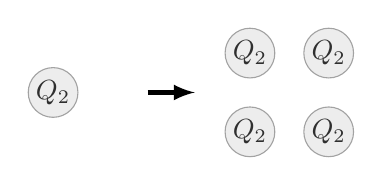
\begin{tikzpicture}[>=latex]
\def\Length{1}
\def\Radius{0.07}

% pre refinement
\LagrangeCell{0}{0}{2*\Length}{\Radius}{2}
{{,,,,,,,,}};
\node[circle, draw=gray, fill=gray!20, inner sep=1pt, opacity=0.7, text opacity=0.8] at (\Length,\Length) {$Q_2$};

% arrow
\draw[->,ultra thick] (2.2*\Length,\Length) -- (2.8*\Length,\Length);

% post refinement
\LagrangeCell{3*\Length}{0}{\Length}{\Radius}{2}
{{,,,,,,,,}};
\node[circle, draw=gray, fill=gray!20, inner sep=1pt, opacity=0.7, text opacity=0.8] at (3.5*\Length,0.5*\Length) {$Q_2$};

\LagrangeCell{4*\Length}{0}{\Length}{\Radius}{2}
{{,,,,,,,,}};
\node[circle, draw=gray, fill=gray!20, inner sep=1pt, opacity=0.7, text opacity=0.8] at (4.5*\Length,0.5*\Length) {$Q_2$};

\LagrangeCell{3*\Length}{\Length}{\Length}{\Radius}{2}
{{,,,,,,,,}};
\node[circle, draw=gray, fill=gray!20, inner sep=1pt, opacity=0.7, text opacity=0.8] at (3.5*\Length,1.5*\Length) {$Q_2$};

\LagrangeCell{4*\Length}{\Length}{\Length}{\Radius}{2}
{{,,,,,,,,}};
\node[circle, draw=gray, fill=gray!20, inner sep=1pt, opacity=0.7, text opacity=0.8] at (4.5*\Length,1.5*\Length) {$Q_2$};
\end{tikzpicture}
\caption{\hp{} refinement}
\end{figure}

\begin{figure}
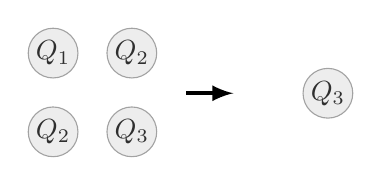
\begin{tikzpicture}[>=latex]
\def\Length{1}
\def\Radius{0.07}

% pre coarsening
\LagrangeCell{0}{0}{\Length}{\Radius}{2}
{{,,,,,,,,}};
\node[circle, draw=gray, fill=gray!20, inner sep=1pt, opacity=0.7, text opacity=0.8] at (0.5\Length,0.5\Length) {$Q_2$};

\LagrangeCell{\Length}{0}{\Length}{\Radius}{3}
{{,,,,,,,,,,,,,,,}};
\node[circle, draw=gray, fill=gray!20, inner sep=1pt, opacity=0.7, text opacity=0.8] at (1.5\Length,0.5\Length) {$Q_3$};

\LagrangeCell{0}{\Length}{\Length}{\Radius}{1}
{{,,,}};
\node[circle, draw=gray, fill=gray!20, inner sep=1pt, opacity=0.7, text opacity=0.8] at (0.5\Length,1.5\Length) {$Q_1$};

\LagrangeCell{\Length}{\Length}{\Length}{\Radius}{2}
{{,,,,,,,,}};
\node[circle, draw=gray, fill=gray!20, inner sep=1pt, opacity=0.7, text opacity=0.8] at (1.5\Length,1.5\Length) {$Q_2$};

% arrow
\draw[->,ultra thick] (2.2*\Length,\Length) -- (2.8*\Length,\Length);

% post coarsening
\LagrangeCell{3*\Length}{0}{2*\Length}{\Radius}{3}
{{,,,,,,,,,,,,,,,}};
\node[circle, draw=gray, fill=gray!20, inner sep=1pt, opacity=0.7, text opacity=0.8] at (4*\Length,\Length) {$Q_3$};
\end{tikzpicture}
\caption{\hp{} coarsening}
\end{figure}
\end{frame}
\begin{frame}
\frametitle{Enumeration of degrees of freedom}

\begin{itemize}
\item Numbering of DoFs necessary to build linear equation
\item Parallelization and p-adaptive methods require different algorithms
  \begin{itemize}
  \item See parallel \parencite{bangerth2012} and hp \cite{bangerth2009} papers for details
  \end{itemize}
\end{itemize}

\vspace{-.7em}
\begin{block}{\vspace{-.7em}}
\centering
Combination of both algorithms \textbf{not trivial}
\end{block}

\vfill{}

\begin{itemize}
\item Why not number DoFs locally and handle relations with constraints?
  \begin{itemize}
  \item Number of DoFs would vary with number of processors
  \item Larger matrices \& vectors, thus higher memory demand
  \end{itemize}
\end{itemize}

\vfill{}

\begin{itemize}
  \item Need for algorithm independent of number of processors
  \begin{itemize}
    \item Results independent of number of processors
    \begin{itemize}
      \item Proof that solvers work
    \end{itemize}
    \item Simplifies debugging
  \end{itemize}
\end{itemize}
\end{frame}





\begin{frame}
\frametitle{Enumeration algorithm}

\begin{itemize}
\item Developed 6-phase algorithm
  \begin{itemize}
  \item Requires two ghost exchanges
  \end{itemize}
\end{itemize}

\vfill{}

\begin{enumerate}
  \item Local enumeration of DoFs
  \item Invalidate DoFs on ghost interfaces to processors with lower rank
  \item Unification of DoFs on local domain \textbf{and} ghost interfaces
  \begin{itemize}
    \item Ownership of DoFs clarified
  \end{itemize}
  \item Global re-enumeration of DoFs
  \begin{itemize}
    \item Local DoF indices set
  \end{itemize}
  \item Exchange of locally owned DoFs
  \item Merge DoFs on ghost interfaces
  \begin{itemize}
    \item Global DoF indices set
  \end{itemize}
\end{enumerate}
\end{frame}




\let\oldthesubfigure\thesubfigure
\renewcommand{\thesubfigure}{Phase \arabic{subfigure}}

\def\Length{1}
\def\Radius{0.03}

\begin{frame}
\frametitle{Example of application of enumeration algorithm}
\begin{overprint}

\onslide<1>
\begin{figure}
  \begin{subfigure}{0.5\textwidth}
    \resizebox{\textwidth}{!}{
      \begin{tikzpicture}[scale=3.3]
  \fill[fzjlightblue] (0, 0) rectangle (2*\Length, \Length);
  \fill[fzjorange] (0, \Length) rectangle (2*\Length, 2*\Length);
  \node at (\Length, 0.7*\Length) {\Huge \textcolor{fzjblue}{\textbf{CPU 0}}};
  \node at (\Length, 1.7*\Length) {\Huge \textcolor[rgb]{0.44,0.26,0.08}{\textbf{CPU 1}}};

  \node at (0.5*\Length, 0.3*\Length) {\Huge \(Q_2\)}; 
  \node at (1.5*\Length, 0.3*\Length) {\Huge \(Q_4\)};
  \node at (0.5*\Length, 1.3*\Length) {\Huge \(Q_4\)}; 
  \node at (1.5*\Length, 1.3*\Length) {\Huge \(Q_2\)};

  \LagrangeCell{0}{0}{\Length}{\Radius}{1}
    {{"","","",""}};
  \LagrangeCell{\Length}{0}{\Length}{\Radius}{1}
    {{"","","",""}};
  \LagrangeCell{0}{\Length}{\Length}{\Radius}{1}
    {{"","","",""}};
  \LagrangeCell{\Length}{\Length}{\Length}{\Radius}{1}
    {{"","","",""}};
\end{tikzpicture}
    }
    \caption{Local enumeration}
  \end{subfigure}
  \caption{Example of application of our enumeration algorithm for degrees of freedom}
\end{figure}

\onslide<2>
\begin{figure}
  \begin{subfigure}{\textwidth}
    \resizebox{\textwidth}{!}{
      \input{addendum/figures/phase1_cpu0}
      \hfill{}
      \begin{tikzpicture}[scale=3.3]
  \fill[color=green] (0, \Length) rectangle (2*\Length, 2*\Length);
  
  \LagrangeCell{0}{0}{\Length}{\Radius}{2}
    {{"i","i","i","i","i","i","i","i","i"}};
  \LagrangeCell{\Length}{0}{\Length}{\Radius}{4}
    {{"i","i","i","i","i","i","i","i","i","i","i","i","i","i","i","i","i","i","i","i","i","i","i","i","i"}};
  \LagrangeCell{0}{\Length}{\Length}{\Radius}{4}
    {{0,1,2,3,4,5,6,7,8,9,10,11,12,13,14,15,16,17,18,19,20,21,22,23,24}};
  \LagrangeCell{\Length}{\Length}{\Length}{\Radius}{2}
    {{25,26,27,28,29,30,31,32,33}};
\end{tikzpicture}

    }
    \caption{Local enumeration}
  \end{subfigure}
  \caption{Example of application of our enumeration algorithm for degrees of freedom}
\end{figure}

\onslide<3>
\begin{figure}
  \ContinuedFloat
  \begin{subfigure}{\textwidth}
    \resizebox{\textwidth}{!}{
      \begin{tikzpicture}[scale=3.3]
  \LagrangeCell{0}{0}{\Length}{\Radius}{2}
    {{0,1,2,3,4,5,6,7,8}};
  \LagrangeCell{\Length}{0}{\Length}{\Radius}{4}
    {{9,10,11,12,13,14,15,16,17,18,19,20,21,22,23,24,25,26,27,28,29,30,31,32,33}};
  \LagrangeCell{0}{\Length}{\Length}{\Radius}{4}
    {{"i","i","i","i","i","i","i","i","i","i","i","i","i","i","i","i","i","i","i","i","i","i","i","i","i"}};
  \LagrangeCell{\Length}{\Length}{\Length}{\Radius}{2}
    {{"i","i","i","i","i","i","i","i","i","i","i","i","i","i","i","i"}};
\end{tikzpicture}
      \hfill{}
      \begin{tikzpicture}[scale=3.3]
  \fill[fzjyellow] (\Length - 0.15, \Length) rectangle (\Length + 0.15, \Length + 0.15);
  
  \LagrangeCell{0}{0}{\Length}{\Radius}{2}
    {{"i","i","i","","i","i","i","i","i"}};
  \LagrangeCell{\Length}{0}{\Length}{\Radius}{4}
    {{"i","i","","i","i","i","i","i","i","i","i","i","i","i","i","i","i","i","i","i","i","i","i","i","i"}};
  \LagrangeCell{0}{\Length}{\Length}{\Radius}{4}
    {{0,"i",2,3,4,5,6,7,8,9,10,11,12,13,14,15,16,17,18,19,20,21,22,23,24}};
  \LagrangeCell{\Length}{\Length}{\Length}{\Radius}{2}
    {{"i",26,27,28,29,30,31,32,33}};
\end{tikzpicture}
    }
    \caption{Invalidation}
  \end{subfigure}
  \caption{Example of application of our enumeration algorithm for degrees of freedom}
\end{figure}

\onslide<4>
\begin{figure}
  \ContinuedFloat
  \begin{subfigure}{\textwidth}
    \resizebox{\textwidth}{!}{
      \begin{tikzpicture}[scale=3.3]
  \fill[color=Set1-F!80] (\Length - 0.15, 0) rectangle (\Length + 0.15, 0.15);
  \fill[color=Set1-F!80] (\Length - 0.15, 0.5*\Length - 0.1) rectangle (\Length + 0.15, 0.5*\Length + 0.1);
  \fill[color=Set1-F!80] (\Length - 0.15, \Length - 0.15) rectangle (\Length + 0.15, \Length);
  
  \fill[color=Set1-F!80] (1.5*\Length - 0.1, \Length - 0.13) rectangle (1.5*\Length + 0.1, \Length + 0.13);
  \fill[color=Set1-F!80] (2*\Length - 0.15, \Length - 0.13) rectangle (2*\Length, \Length + 0.13);
  
  \LagrangeCell{0}{0}{\Length}{\Radius}{2}
    {{0,1,2,3,4,5,6,7,8}};
  \LagrangeCell{\Length}{0}{\Length}{\Radius}{4}
    {{1,10,3,"i",13,5,15,16,17,18,19,20,21,22,"i",24,25,26,27,28,29,30,31,32,33}};
  \LagrangeCell{0}{\Length}{\Length}{\Radius}{4}
    {{"i","i","i","i","i","i","i","i","i","i","i","i","i","i","i","i","i","i","i","i","i","i","i","i","i"}};
  \LagrangeCell{\Length}{\Length}{\Length}{\Radius}{2}
    {{"i","i","i","i","i","i","i","i","i","i","i","i","i","i","i","i"}};
\end{tikzpicture}
      \hfill{}
      \begin{tikzpicture}[scale=3.3]
  \fill[fzjyellow] (\Length - 0.15, 1.5*\Length - 0.1) rectangle (\Length + 0.15, 1.5*\Length + 0.1);
  \fill[fzjyellow] (\Length - 0.15, 2*\Length - 0.15) rectangle (\Length + 0.15, 2*\Length);
  
  \fill[fzjyellow] (0, \Length - 0.13) rectangle (0.15, \Length + 0.13);
  \fill[fzjyellow] (0.5*\Length - 0.1, \Length - 0.13) rectangle (0.5*\Length + 0.1, \Length + 0.13);
  
  \LagrangeCell{0}{0}{\Length}{\Radius}{2}
    {{"i","i","i","","i","i","i","i","i"}};
  \LagrangeCell{\Length}{0}{\Length}{\Radius}{4}
    {{"i","i","","i","i","i","i","i","i","i","i","i","i","i","i","i","i","i","i","i","i","i","i","i","i"}};
  \LagrangeCell{0}{\Length}{\Length}{\Radius}{4}
    {{"i","i",2,27,4,5,6,7,29,9,10,"i",12,13,14,15,16,17,18,19,20,21,22,23,24}};
  \LagrangeCell{\Length}{\Length}{\Length}{\Radius}{2}
    {{"i",26,27,28,29,30,31,32,33}};
\end{tikzpicture}
    }
    \caption{Unification}
  \end{subfigure}
  \caption{Example of application of our enumeration algorithm for degrees of freedom}
\end{figure}

\onslide<5>
\begin{figure}
  \ContinuedFloat
  \begin{subfigure}{\textwidth}
    \resizebox{\textwidth}{!}{
      \begin{tikzpicture}[scale=3.3]
  \fill[fzjyellow] (0, 0) rectangle (2*\Length, \Length);
  
  \fill[white] (1.5*\Length - 0.1, \Length - 0.13) rectangle (1.5*\Length + 0.1, \Length + 0.13);
  \fill[white] (2*\Length - 0.15, \Length - 0.13) rectangle (2*\Length, \Length + 0.13);
  
  \LagrangeCell{0}{0}{\Length}{\Radius}{2}
    {{0,1,2,3,4,5,6,7,8}};
  \LagrangeCell{\Length}{0}{\Length}{\Radius}{4}
    {{1,9,3,"i",10,5,11,12,13,14,15,16,17,18,"i",19,20,21,22,23,24,25,26,27,28}};
  \LagrangeCell{0}{\Length}{\Length}{\Radius}{4}
    {{"i","","i","i","i","i","i","i","i","i","i","i","i","i","i","i","i","i","i","i","i","i","i","i","i"}};
  \LagrangeCell{\Length}{\Length}{\Length}{\Radius}{2}
    {{"","i","i","i","i","i","i","i","i","i","i","i","i","i","i","i"}};
\end{tikzpicture}
      \hfill{}
      \begin{tikzpicture}[scale=3.3]
  \fill[fzjyellow] (0, \Length) rectangle (2*\Length, 2*\Length);
  
  \fill[white] (\Length - 0.15, \Length) rectangle (\Length + 0.15, \Length + 0.15);
  \fill[white] (0, \Length - 0.13) rectangle (0.15, \Length + 0.13);
  \fill[white] (0.5*\Length - 0.1, \Length - 0.13) rectangle (0.5*\Length + 0.1, \Length + 0.13);
  
  \LagrangeCell{0}{0}{\Length}{\Radius}{2}
    {{"i","i","i","","i","i","i","i","i"}};
  \LagrangeCell{\Length}{0}{\Length}{\Radius}{4}
    {{"i","i","","i","i","i","i","i","i","i","i","i","i","i","i","i","i","i","i","i","i","i","i","i","i"}};
  \LagrangeCell{0}{\Length}{\Length}{\Radius}{4}
    {{"i","i",29,30,31,32,33,34,35,36,37,"i",38,39,40,41,42,43,44,45,46,47,48,49,50}};
  \LagrangeCell{\Length}{\Length}{\Length}{\Radius}{2}
    {{"i",51,30,52,35,53,54,55,56}};
\end{tikzpicture}
    }
    \caption{Re-enumeration}
  \end{subfigure}
  \caption{Example of application of our enumeration algorithm for degrees of freedom}
\end{figure}

\onslide<6>
\begin{figure}
  \ContinuedFloat
  \begin{subfigure}{\textwidth}
    \resizebox{\textwidth}{!}{
      \begin{tikzpicture}[scale=3.3]
  \fill[color=green] (0,\Length) rectangle (2*\Length, 2*\Length);
  
  \fill[white] (\Length - 0.15, \Length) rectangle (\Length + 0.15, \Length + 0.15);
  \fill[white] (0, \Length - 0.13) rectangle (0.15, \Length + 0.13);
  \fill[white] (0.5*\Length - 0.1, \Length - 0.13) rectangle (0.5*\Length + 0.1, \Length + 0.13);
  
  \LagrangeCell{0}{0}{\Length}{\Radius}{2}
    {{0,1,2,3,4,5,6,7,8}};
  \LagrangeCell{\Length}{0}{\Length}{\Radius}{4}
    {{1,9,3,"i",10,5,11,12,13,14,15,16,17,18,"i",19,20,21,22,23,24,25,26,27,28}};
  \LagrangeCell{0}{\Length}{\Length}{\Radius}{4}
    {{"i","i",29,50,30,31,32,33,52,34,35,"i",36,37,38,39,40,41,42,43,44,45,46,47,48}};
  \LagrangeCell{\Length}{\Length}{\Length}{\Radius}{2}
    {{"i",49,50,51,52,53,54,55,56}};
\end{tikzpicture}
      \hfill{}
      \input{addendum/figures/phase5_cpu1}
    }
    \caption{Ghost exchange}
  \end{subfigure}
  \caption{Example of application of our enumeration algorithm for degrees of freedom}
\end{figure}

\onslide<7>
\begin{figure}
  \ContinuedFloat
  \begin{subfigure}{\textwidth}
    \resizebox{\textwidth}{!}{
      \input{addendum/figures/phase6_cpu0}
      \hfill{}
      \begin{tikzpicture}[scale=3.3]
  \fill[color=green] (0, \Length - 0.13) rectangle (0.15, \Length + 0.13);
  \fill[color=green] (0.5*\Length - 0.1, \Length - 0.13) rectangle (0.5*\Length + 0.1, \Length + 0.13);
  \fill[color=green] (1.5*\Length - 0.1, \Length - 0.13) rectangle (1.5*\Length + 0.1, \Length + 0.13);
  \fill[color=green] (2*\Length - 0.15, \Length - 0.13) rectangle (2*\Length, \Length + 0.13);
  
  \LagrangeCell{0}{0}{\Length}{\Radius}{2}
    {{0,1,2,"",4,5,6,7,8}};
  \LagrangeCell{\Length}{0}{\Length}{\Radius}{4}
    {{1,9,"",51,10,5,11,12,13,14,15,16,17,18,54,19,20,21,22,23,24,25,26,27,28}};
  \LagrangeCell{0}{\Length}{\Length}{\Radius}{4}
    {{2,3,29,30,31,32,33,34,35,36,37,7,38,39,40,41,42,43,44,45,46,47,48,49,50}};
  \LagrangeCell{\Length}{\Length}{\Length}{\Radius}{2}
    {{3,51,30,52,35,53,54,55,56}};
\end{tikzpicture}

    }
    \caption{Merge}
  \end{subfigure}
  \caption{Example of application of our enumeration algorithm for degrees of freedom}
\end{figure}

\end{overprint}
\end{frame}

\renewcommand{\thesubfigure}{\oldthesubfigure}
\begin{frame}
\frametitle{Data transfer across subdomains}

\begin{itemize}
\item On distributed triangulations, each subdomain needs access to relevant fraction of global quantities
\item Changes on cell ownership requires transfer of these quantities
  \begin{itemize}
  \item Active finite element indices
  \item Solution
  \item ...
  \end{itemize}
\item With p-adaptive methods, per cell data sizes may differ
\end{itemize}

\vspace{-.7em}
\begin{block}{\vspace{-.7em}}
  \centering
  Communication between involved processors required
\end{block}

\vfill{}

\begin{itemize}
\item Algorithm should be generic, i.e.\@ independent of scenario
  \begin{enumerate}
  \item Creation of \textbf{memory buffers}
  \item Transfer data of \textbf{fixed} and \textbf{variable} size
  \end{enumerate}
\end{itemize}
\end{frame}





\begin{frame}
\frametitle{Structure of memory buffers}

\begin{itemize}
\item Register functions that prepare data to be transferred via callback
\end{itemize}

\vfill{}

\begin{itemize}
\item \textbf{On each locally owned cell}:
  \begin{enumerate}
  \item Pack data for each registered callback individually
  \item Store memory sizes of each callback's data pack
  \item Store memory size of cell's complete data pack
  \end{enumerate}
\item \textbf{After each cell} is processed:
  \begin{enumerate}
  \setcounter{enumi}{3}
  \item Move each cell's packed data into contiguous buffer
  \end{enumerate}
\end{itemize}

\vfill{}

\begin{figure}
\begin{tikzpicture}[scale=0.7]
% draw cells
\draw[fill=fzjlightblue] (0,-0.5) rectangle ( 7,2);
\draw[fill=fzjorange]    (7,-0.5) rectangle (14,2);
\node[align=center] at ( 3.5, 1.6) {cell\textunderscore{}1};
\node[align=center] at (10.5, 1.6) {cell\textunderscore{}2};
\node[align=center] at (14.5, 1.6) {...};

% draw callbacks
% cell_1
\draw[fill=fzjred]   (0,-0.25) rectangle (3,1.25);
\draw[fill=fzjgreen] (3,-0.25) rectangle (6,1.25);
\node[align=center] at (1.5,0.85) {callback\textunderscore{}1};
\node[align=center] at (4.5,0.85) {callback\textunderscore{}2};
\node[align=center] at (6.5,0.85) {...};
% cell_2
\draw[fill=fzjred]   ( 7,-0.25) rectangle (10,1.25);
\draw[fill=fzjgreen] (10,-0.25) rectangle (13,1.25);
\node[align=center] at ( 8.5,0.85) {callback\textunderscore{}1};
\node[align=center] at (11.5,0.85) {callback\textunderscore{}2};
\node[align=center] at (13.5,0.85) {...};
% beyond
\node[align=center] at (14.5,0.85) {...};

% draw contiguous memory
\draw[fill=white] (-1,0) rectangle (15,0.5);
\foreach \x in {0,...,14}
\draw (\x,0) -- (\x,0.5);
% cell_1
\node[align=center] at ( 2.5,0.25) {...};
\node[align=center] at ( 5.5,0.25) {...};
\node[align=center] at ( 6.5,0.25) {...};
% cell_2
\node[align=center] at ( 9.5,0.25) {...};
\node[align=center] at (12.5,0.25) {...};
\node[align=center] at (13.5,0.25) {...};
% beyond
\node[align=center] at (-0.5,0.25) {...};
\node[align=center] at (14.5,0.25) {...};
\end{tikzpicture}
\caption{Division of contiguous memory chunk}
\end{figure}
\end{frame}





\begin{frame}
\frametitle{Data consignment}

\begin{itemize}
  \item Treat fixed and variable size data separately
  \begin{itemize}
    \item Each transfer algorithm optimized for their specific task
    \item Potentially slower variable size transfer will only be used when necessary
  \end{itemize}
\end{itemize}

\vfill{}

\begin{enumerate}
\item \textbf{Fixed size data}:
  \begin{itemize}
  \item Refrain from using compression
  \item Additionally pack \texttt{CellStatus} information
  \item Gathering callback sizes on first packed cell will suffice
    \begin{itemize}
    \item Communicate callback sizes to all processors
    \end{itemize}
  \end{itemize}
  \item \textbf{Variable size data}:
  \begin{itemize}
  \item Compression allowed (using \texttt{ZLIB})
  \item Size of each callback's data differs from cell to cell
    \begin{itemize}
    \item Register additional callback for fixed size data transfer
    \end{itemize}
  \end{itemize}
\end{enumerate}
\end{frame}





\begin{frame}
\frametitle{Data transfer}

\begin{itemize}
\item We have contiguous memory chunks for data transfer during\\ repartitioning, refinement/coarsening, serialization
  \begin{itemize}
  \item Program may be resumed with a different number of processors
  \end{itemize}
\end{itemize}

\vfill

\begin{itemize}
\item Data consignment \textbf{independent} of transfer algorithms used for\\ repartitioning, refinement/coarsening, serialization
  \begin{itemize}
  \item Use non-blocking \texttt{MPI} communication for all operations
  \item \dealii{} utilizes interface to \pforest{} \cite{burstedde}
  \end{itemize}
\end{itemize}
\end{frame}
\begin{frame}
\frametitle{FEM error behavior}

\begin{itemize}
\item Error behavior for \hp-FEM is well understood \parencite{babuska1990}
  \begin{align*}
  \left\|\nabla\left(u \!-\! u_\text{hp}\right)\right\|_{H^{1}(\Omega)} &\leq C \, \frac{h^p}{p^{m-1}} \, \|u\|_{H^{m}(\Omega)}
  \end{align*}
\end{itemize}

\begin{itemize}
\item Exponential convergence rate possible with \hp-adaptation \parencite{babuska1996}
  \begin{align*}
  \left\|\nabla\left(u \!-\! u_\text{hp}\right)\right\|_{H^{1}(\Omega)} &\leq C \, \exp\left(- b \, N_\text{dofs}^\alpha\right)
  \end{align*}
  with $\alpha = 1/3$ in 2D and $\alpha = 1/5$ in 3D
\end{itemize}
\end{frame}





\begin{frame}
\frametitle{Kelly error estimation}

\begin{itemize}
\item Error estimator by \parencite{kelly1983}
\item Meant for generalized Poisson equation $-\nabla \cdot (a \nabla u) = f$
\item Proved to be useful in other applications as well
\end{itemize}

\begin{align*}
\|e_\text{hp}\|_{H_1(\Omega)}^2 &\leq C \sum\limits_{K \in \Omega} \eta_K^2 \\
\eta_K^2 &= \sum\limits_{F \in \partial K} c_F \int\limits_{F} \left[ a \, \frac{\partial u_\text{hp}}{\partial n} \right]^2 do \\
\left[ a \, \frac{\partial u_\text{hp}}{\partial n} \right] &= \left. a \, \frac{\partial u_\text{hp}}{\partial n_K} \right|_K + \left. a \, \frac{\partial u_\text{hp}}{\partial n_J}\right|_J
\end{align*}
\end{frame}





\begin{frame}
\frametitle{Refinement history}

\begin{minipage}{.56\textwidth}
  \begin{itemize}
    \item Verify prediction's accuracy
    \item Decide on either h- or p-adaptation on marked cells\\[.4em]
    \begin{tabular}{ll}
      Keep \textbf{\h} small: & $\eta_K > \eta_{K,\text{pred}}$ \\
      Keep \textbf{\p} large: & $\eta_K \leq \eta_{K,\text{pred}}$
    \end{tabular}
  \end{itemize}
\end{minipage}
\begin{minipage}{.43\textwidth}
  \begin{figure}
    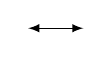
\begin{tikzpicture}[scale=0.7]
    \def\Radius{.09}
    \LagrangeCell{-4}{0}{2}{\Radius}{1}{{,,,}};
    
    \draw[>=latex, <->] (-1.5,1) -- (-.5,1);
    
    \LagrangeCell{0}{0}{1}{\Radius}{1}{{,,,}};
    \LagrangeCell{0}{1}{1}{\Radius}{1}{{,,,}};
    \LagrangeCell{1}{0}{1}{\Radius}{1}{{,,,}};
    \LagrangeCell{1}{1}{1}{\Radius}{1}{{,,,}};
    \end{tikzpicture}
    \caption{\h-adaptation}
  \end{figure}
\end{minipage}

\begin{table}
\caption{Error prediction algorithm based on \parencite{melenk2001}}
\vspace{-1em}
\begin{tabular}{ll}
  \rowcolor{fzjblue!25} \multicolumn{1}{c}{\textbf{Adaptation type}} & \multicolumn{1}{c}{\textbf{Prediction formula}} \\
  \toprule
  no adaptation & $\eta_{K,\text{pred}} = \eta_{K} \, \gamma_\text{n}$ \\
  \midrule
  \p-adaptation & $\eta_{K,\text{pred}} = \eta_{K} \,
\gamma_\text{p}^{(p_{K,\text{future}} - p_K)}$ \\
  \midrule
  \hp-refinement & $\left( \eta_{K_c,\text{pred}} \right)^2 = n_{K_c}^{-1}
\left( \eta_{K_p} \,
\gamma_\text{h} \, 0.5^{p_{K_c,\text{future}}} \,
\gamma_\text{p}^{(p_{K_c,\text{future}} - p_{K_p})} \right)^2$ \\
  \addlinespace[1mm]
  \hp-coarsening & $\left( \eta_{K_p,\text{pred}} \right)^2 = \sum\limits_{K_c} \left( \eta_{K_c} \,
(\gamma_\text{h} \, 0.5^{p_{K_p,\text{future}}})^{-1} \, \gamma_\text{p}^{(p_{K_p,\text{future}} - p_{K_c})} \right)^2$
\end{tabular}
\end{table}
\end{frame}





\begin{frame}
\frametitle{Smoothness estimation}

\begin{itemize}
\item Different representations of finite element approximation
\begin{align*}
u_{hp}(x) = \sum\limits_i u_i \, \varphi_i(x)  = \sum\limits_k c_k \, P_k(x)
\end{align*}
\end{itemize}

\begin{itemize}
\item Choose orthogonal basis $\{P_k\}$ of increasing frequency
\item Uniquely attribute frequency of oscillations to each basis function
\end{itemize}
\end{frame}





\begin{frame}
\frametitle{Orthogonal basis}

\begin{itemize}
\item Legendre: Orthogonal basis of polynomials
  \begin{align*}
  P_k(x) &= \frac{1}{2^k k!} \frac{d^k}{dx^k} \left( (x^2 - 1)^k \right) \\
  \langle P_k, P_l \rangle &= \int P_k(x) \, P_l(x) \, dx = \frac{2}{2k+1} \delta_{kl}
  \end{align*}
\end{itemize}

\begin{itemize}
\item Fourier: Orthogonal basis of sinusoids
  \begin{align*}
  P_k(x) &= \exp \left( -i \, 2 \pi k \, x \right) \\
  \langle P_k, P_l \rangle &= \int P_k(x) \, P_l^*(x) \, dx = \delta_{kl}
  \end{align*}
\end{itemize}
\end{frame}





\begin{frame}
\frametitle{Legendre polynomials}

\begin{tikzpicture}
\begin{axis}[
%cycle list/Dark2,
scale=.97,
ymin=-1.2, ymax=1.2,
xlabel=$x$,
ylabel=$P_k(x)$,
grid=major,
%legend style={at={(0.5,1.02)}, anchor=south, /tikz/every even column/.append style={column sep=0.5cm}},
%legend columns=3,
legend cell align=left,
legend pos = outer north east,
legend style={font=\tiny},
cycle list/Dark2,
every axis plot/.append style={ultra thick}
]
\addplot+[samples=2, domain=-1:1] {1};
\addlegendentry{$P_0 = 1$};

\only<2->{
\addplot+[samples=2, domain=-1:1] {x};
\addlegendentry{$P_1 = x$};
}

\only<3->{
\addplot+[samples=20, domain=-1:1] {0.5*(3*x^2-1)};
\addlegendentry{$P_2 = \frac{1}{2} \left( 3x^2 - 1 \right)$};
}

\only<4->{
\addplot+[samples=40, domain=-1:1] {0.5*(5*x^3 - 3*x)};
\addlegendentry{$P_3 = \frac{1}{2} \left( 5x^3 - 3x \right)$};
}

\only<5->{
\addplot+[samples=60, domain=-1:1] {0.125*(35*x^4 - 30*x^2 + 3)};
\addlegendentry{$P_4 = \frac{1}{8} \left( 35x^4 - 30x^2 + 3 \right)$};
}

\only<6->{
\addplot+[samples=80, domain=-1:1] {0.125*(63*x^5 - 70*x^3 + 15*x)};
\addlegendentry{$P_5 = \frac{1}{8} \left( 63x^5 - 70x^3 + 15x \right)$};
}
\end{axis}
\end{tikzpicture}
\end{frame}





\begin{frame}
\frametitle{Fourier sinusoids}

\begin{tikzpicture}
\begin{axis}[
%cycle list/Dark2,
scale=.97,
ymin=-1.2, ymax=1.2,
xlabel=$x$,
ylabel=$\operatorname{Re}\left(P_k(x)\right)$,
grid=major,
%legend style={at={(0.5,1.02)}, anchor=south, /tikz/every even column/.append style={column sep=0.5cm}},
%legend columns=3,
legend cell align=left,
legend pos = outer north east,
legend style={font=\tiny},
cycle list/Dark2,
every axis plot/.append style={ultra thick}
]
\addplot+[samples=2, domain=0:1] {1};
\addlegendentry{$P_0 = 1$};

\only<2->{
\addplot+[samples=30, domain=0:1] {cos(deg(6.28*x))};
\addlegendentry{$P_1 = \exp\left(i \, 2\pi \, x\right)$};
}

\only<3->{
\addplot+[samples=60, domain=0:1] {cos(deg(2*6.28*x))};
\addlegendentry{$P_2 = \exp\left(i \, 4\pi \, x\right)$};
}

\only<4->{
\addplot+[samples=90, domain=0:1] {cos(deg(3*6.28*x))};
\addlegendentry{$P_3 = \exp\left(i \, 6\pi \, x\right)$};
}

\only<5->{
\addplot+[samples=120, domain=0:1] {cos(deg(4*6.28*x))};
\addlegendentry{$P_4 = \exp\left(i \, 8\pi \, x\right)$};
}
\end{axis}
\end{tikzpicture}
\end{frame}





\begin{frame}
\frametitle{Decay of Legendre coefficients}

\begin{itemize}
\item Determine coefficients $\{c_k\}$ on every cell $K$:
  \begin{align*}
  c_k = \int\limits_K u_{hp}(x) \, P_k(x) \, dx
  \end{align*}
  
\item FE approximation is analytic if coefficients decay exponentially \cite{eibner2007}
  \begin{align*}
  |c_k| \leq C \exp\left( - \sigma |k| \right)
  \end{align*}
  
\item Determine decay rate $\sigma$ via least-squares fit
  \begin{align*}
  \ln(|c_k|) \sim \tilde{C} - \sigma |k|
  \end{align*}
\end{itemize}

\vspace{-1em}
\begin{block}{\vspace{-1em}}
\centering
Decay rates $\sigma$ considered as smoothness estimates \\
Keep $p$ large if $\sigma$ is large
\end{block}
\vspace{1em}
\end{frame}





\begin{frame}
\frametitle{Decay of Fourier coefficients}

\begin{itemize}
\item FE approximation is part of Hilbert space $\mathcal{H}^s$ if integral exists
  \begin{align*}
  \int\limits_K \left| \nabla^s u_{\text{hp}}(x) \right|^2 dx &= (2 \pi)^{2s} \sum\limits_k \left| c_k \right|^2 k^{2s} < \infty \\
  \Rightarrow\qquad |c_k| = \mathcal{O}&\left(k^{-\sigma - \epsilon}\right)  \quad \text{with} \quad \sigma = s + \text{dim}/2
  \end{align*}

\item Determine coefficients $\{c_k\}$ and their decay via least-squares fit on every cell $K$:
  \begin{align*}
  c_k &= \int\limits_K u_{hp}(x) \, P_k^*(x) \, dx & \ln(|c_k|) &\sim C - \sigma \ln\left( |k| \right)
  \end{align*}
\end{itemize}

\vspace{-1em}
\begin{block}{\vspace{-1em}}
\centering
Decay rates $\sigma$ considered as smoothness estimates \\
Keep $p$ large if $\sigma$ is large
\end{block}
\vspace{1em}
\end{frame}

\subtitle{More results}
\maketitle
\section{Error versus performance}
\label{sec:errorvsperformance}

Text.

\begin{figure}
\centering
\begin{tikzpicture}
\begin{loglogaxis}[
  xlabel=Number of \glspl{dof},
  ylabel=H1 error]
\addplot table [y=H1 error, x=ndofs, col sep=comma] {data/error/h.csv};
\addplot table [y=H1 error, x=ndofs, col sep=comma] {data/error/p.csv};
\addplot table [y=H1 error, x=ndofs, col sep=comma] {data/error/hp-legendre.csv};
\addplot table [y=H1 error, x=ndofs, col sep=comma] {data/error/hp-fourier.csv};
\addplot table [y=H1 error, x=ndofs, col sep=comma] {data/error/hp-prediction.csv};
\addplot table [y=H1 error, x=ndofs, col sep=comma] {data/error/hp-legendre-naive.csv};
\addplot table [y=H1 error, x=ndofs, col sep=comma] {data/error/hp-fourier-naive.csv};
\addplot table [y=H1 error, x=ndofs, col sep=comma] {data/error/hp-prediction-naive.csv};
\end{loglogaxis}
\end{tikzpicture}
\caption{Error vs workload.}
\label{fig:errorworkload}
\end{figure}

\begin{figure}
\centering
\begin{tikzpicture}
\begin{loglogaxis}[
  xlabel=Wall time {[seconds]},
  ylabel=H1 error,
  legend pos=outer north east]
\addplot table [y=H1 error, x=walltime, col sep=comma] {data/error/h.csv};
\addlegendentry{\h};

\addplot table [y=H1 error, x=walltime, col sep=comma] {data/error/p.csv};
\addlegendentry{\p};

\addplot table [y=H1 error, x=walltime, col sep=comma] {data/error/hp-legendre.csv};
\addlegendentry{\hp{} Legendre};

\addplot table [y=H1 error, x=walltime, col sep=comma] {data/error/hp-fourier.csv};
\addlegendentry{\hp{} Fourier};

\addplot table [y=H1 error, x=walltime, col sep=comma] {data/error/hp-prediction.csv};
\addlegendentry{\hp{} Prediction};

\addplot table [y=H1 error, x=walltime, col sep=comma] {data/error/hp-legendre-naive.csv};
\addlegendentry{\hp{} Legendre naive};

\addplot table [y=H1 error, x=walltime, col sep=comma] {data/error/hp-fourier-naive.csv};
\addlegendentry{\hp{} Fourier naive};

\addplot table [y=H1 error, x=walltime, col sep=comma] {data/error/hp-prediction-naive.csv};
\addlegendentry{\hp{} Prediction naive};
\end{loglogaxis}
\end{tikzpicture}
\caption{Error vs walltime.}
\label{fig:errorwalltime}
\end{figure}
\begin{frame}
\frametitle{Weighting exponent}

\vspace{-1em}
\begin{figure}
\resizebox{!}{.75\textheight}{
  \begin{tikzpicture}
  \begin{groupplot}[
  group style={
    group size=1 by 2,
    vertical sep=0pt
  },
  width=9.5cm,
  grid=major,
  xlabel=Weighting exponent,
  ylabel=Wall time {[seconds]},
  legend cell align=left,
  legend pos=outer north east,
  cycle list/Set1]
  
  
  \nextgroupplot[
  xlabel = {},
  axis x line=top,
  x axis line style={-},
  axis y discontinuity=parallel]
  \addplot[mark=square*, index of colormap=1 of Set1] table [y=full cycle, x=weighting exponent, col sep=comma] {data/weight/weight.csv};
  \addlegendentry{full cycle};
  
  \addplot[mark=*, index of colormap=2 of Set1] table [y=solve, x=weighting exponent, col sep=comma] {data/weight/weight.csv};
  \addlegendentry{linear solver};
  
  \addlegendimage{mark=triangle*, index of colormap=3 of Set1};
  \addlegendentry{assemble linear system};
  
  
  \nextgroupplot[
  ymax = 21,
  ytick={10,20},
  axis x line=bottom,
  x axis line style={-},
  ylabel={},
  height=3.1cm
  ]
  \addplot[mark=triangle*, index of colormap=3 of Set1] table [y=assembly, x=weighting exponent, col sep=comma] {data/weight/weight.csv};
  \end{groupplot}
  \end{tikzpicture}
}
\caption{Wall times for load balancing with varying weighting exponents}
\end{figure}
\end{frame}
\begin{frame}
\frametitle{Scaling on successive refinement}

\begin{figure}
\hspace*{-0.5em}
\begin{tikzpicture}
\begin{loglogaxis}[
scale=0.9,
xlabel={Number of degrees of freedom},
ylabel={Wall time [seconds]},
grid=major,
legend cell align=left,
legend pos=outer north east,
legend style={font=\tiny}
]

% data
\addplot table [y=solve, x=ndofs, col sep=comma] {data/weak/weak-nodes16.csv};
\addlegendentry{linear solver};

\addplot table [y=setup, x=ndofs, col sep=comma] {data/weak/weak-nodes16.csv};
\addlegendentry{setup data structures};

\addplot table [y=assembly, x=ndofs, col sep=comma] {data/weak/weak-nodes16.csv};
\addlegendentry{assemble linear system};

\addplot table [y=compute errors, x=ndofs, col sep=comma] {data/weak/weak-nodes16.csv};
\addlegendentry{estimate error};

\addplot table [y=calculate indicators, x=ndofs, col sep=comma] {data/weak/weak-nodes16.csv};
\addlegendentry{estimate smoothness};

\addplot table [y=refine, x=ndofs, col sep=comma] {data/weak/weak-nodes16.csv};
\addlegendentry{coarsen and refine};

% optimal line
\addplot[very thick, samples=2, domain=12591105:1302365268] {10^(-7.2)*x};
\addlegendentry{optimal convergence};

% auxiliary lines
\begin{scope}
\draw[green, very thick] ({axis cs:76800000,0}|-{rel axis cs:0,1}) -- ({axis cs:76800000,0}|-{rel axis cs:0,0});
\draw[blue, very thick] ({axis cs:50647318,0}|-{rel axis cs:0,1}) -- ({axis cs:50647318,0}|-{rel axis cs:0,0});
\end{scope}
\addlegendimage{color=green};
\addlegendentry{$10^5$ DoFs per process};
\addlegendimage{color=blue};
\addlegendentry{each reference finite element in mesh};
\end{loglogaxis}
\end{tikzpicture}
\caption{Scaling on successively refined grids}
\end{figure}
\end{frame}

\end{document}
